% Options for packages loaded elsewhere
\PassOptionsToPackage{unicode}{hyperref}
\PassOptionsToPackage{hyphens}{url}
%
\documentclass[
  parskip,
  oneside]{scrreprt}
\title{Schildkrötenkrebs}
\author{}
\date{\vspace{-2.5em}}

\usepackage{amsmath,amssymb}
\usepackage{lmodern}
\usepackage{iftex}
\ifPDFTeX
  \usepackage[T1]{fontenc}
  \usepackage[utf8]{inputenc}
  \usepackage{textcomp} % provide euro and other symbols
\else % if luatex or xetex
  \usepackage{unicode-math}
  \defaultfontfeatures{Scale=MatchLowercase}
  \defaultfontfeatures[\rmfamily]{Ligatures=TeX,Scale=1}
\fi
% Use upquote if available, for straight quotes in verbatim environments
\IfFileExists{upquote.sty}{\usepackage{upquote}}{}
\IfFileExists{microtype.sty}{% use microtype if available
  \usepackage[]{microtype}
  \UseMicrotypeSet[protrusion]{basicmath} % disable protrusion for tt fonts
}{}
\makeatletter
\@ifundefined{KOMAClassName}{% if non-KOMA class
  \IfFileExists{parskip.sty}{%
    \usepackage{parskip}
  }{% else
    \setlength{\parindent}{0pt}
    \setlength{\parskip}{6pt plus 2pt minus 1pt}}
}{% if KOMA class
  \KOMAoptions{parskip=half}}
\makeatother
\usepackage{xcolor}
\IfFileExists{xurl.sty}{\usepackage{xurl}}{} % add URL line breaks if available
\IfFileExists{bookmark.sty}{\usepackage{bookmark}}{\usepackage{hyperref}}
\hypersetup{
  pdftitle={Schildkrötenkrebs},
  hidelinks,
  pdfcreator={LaTeX via pandoc}}
\urlstyle{same} % disable monospaced font for URLs
\usepackage{color}
\usepackage{fancyvrb}
\newcommand{\VerbBar}{|}
\newcommand{\VERB}{\Verb[commandchars=\\\{\}]}
\DefineVerbatimEnvironment{Highlighting}{Verbatim}{commandchars=\\\{\}}
% Add ',fontsize=\small' for more characters per line
\usepackage{framed}
\definecolor{shadecolor}{RGB}{248,248,248}
\newenvironment{Shaded}{\begin{snugshade}}{\end{snugshade}}
\newcommand{\AlertTok}[1]{\textcolor[rgb]{0.94,0.16,0.16}{#1}}
\newcommand{\AnnotationTok}[1]{\textcolor[rgb]{0.56,0.35,0.01}{\textbf{\textit{#1}}}}
\newcommand{\AttributeTok}[1]{\textcolor[rgb]{0.77,0.63,0.00}{#1}}
\newcommand{\BaseNTok}[1]{\textcolor[rgb]{0.00,0.00,0.81}{#1}}
\newcommand{\BuiltInTok}[1]{#1}
\newcommand{\CharTok}[1]{\textcolor[rgb]{0.31,0.60,0.02}{#1}}
\newcommand{\CommentTok}[1]{\textcolor[rgb]{0.56,0.35,0.01}{\textit{#1}}}
\newcommand{\CommentVarTok}[1]{\textcolor[rgb]{0.56,0.35,0.01}{\textbf{\textit{#1}}}}
\newcommand{\ConstantTok}[1]{\textcolor[rgb]{0.00,0.00,0.00}{#1}}
\newcommand{\ControlFlowTok}[1]{\textcolor[rgb]{0.13,0.29,0.53}{\textbf{#1}}}
\newcommand{\DataTypeTok}[1]{\textcolor[rgb]{0.13,0.29,0.53}{#1}}
\newcommand{\DecValTok}[1]{\textcolor[rgb]{0.00,0.00,0.81}{#1}}
\newcommand{\DocumentationTok}[1]{\textcolor[rgb]{0.56,0.35,0.01}{\textbf{\textit{#1}}}}
\newcommand{\ErrorTok}[1]{\textcolor[rgb]{0.64,0.00,0.00}{\textbf{#1}}}
\newcommand{\ExtensionTok}[1]{#1}
\newcommand{\FloatTok}[1]{\textcolor[rgb]{0.00,0.00,0.81}{#1}}
\newcommand{\FunctionTok}[1]{\textcolor[rgb]{0.00,0.00,0.00}{#1}}
\newcommand{\ImportTok}[1]{#1}
\newcommand{\InformationTok}[1]{\textcolor[rgb]{0.56,0.35,0.01}{\textbf{\textit{#1}}}}
\newcommand{\KeywordTok}[1]{\textcolor[rgb]{0.13,0.29,0.53}{\textbf{#1}}}
\newcommand{\NormalTok}[1]{#1}
\newcommand{\OperatorTok}[1]{\textcolor[rgb]{0.81,0.36,0.00}{\textbf{#1}}}
\newcommand{\OtherTok}[1]{\textcolor[rgb]{0.56,0.35,0.01}{#1}}
\newcommand{\PreprocessorTok}[1]{\textcolor[rgb]{0.56,0.35,0.01}{\textit{#1}}}
\newcommand{\RegionMarkerTok}[1]{#1}
\newcommand{\SpecialCharTok}[1]{\textcolor[rgb]{0.00,0.00,0.00}{#1}}
\newcommand{\SpecialStringTok}[1]{\textcolor[rgb]{0.31,0.60,0.02}{#1}}
\newcommand{\StringTok}[1]{\textcolor[rgb]{0.31,0.60,0.02}{#1}}
\newcommand{\VariableTok}[1]{\textcolor[rgb]{0.00,0.00,0.00}{#1}}
\newcommand{\VerbatimStringTok}[1]{\textcolor[rgb]{0.31,0.60,0.02}{#1}}
\newcommand{\WarningTok}[1]{\textcolor[rgb]{0.56,0.35,0.01}{\textbf{\textit{#1}}}}
\usepackage{graphicx}
\makeatletter
\def\maxwidth{\ifdim\Gin@nat@width>\linewidth\linewidth\else\Gin@nat@width\fi}
\def\maxheight{\ifdim\Gin@nat@height>\textheight\textheight\else\Gin@nat@height\fi}
\makeatother
% Scale images if necessary, so that they will not overflow the page
% margins by default, and it is still possible to overwrite the defaults
% using explicit options in \includegraphics[width, height, ...]{}
\setkeys{Gin}{width=\maxwidth,height=\maxheight,keepaspectratio}
% Set default figure placement to htbp
\makeatletter
\def\fps@figure{htbp}
\makeatother
\setlength{\emergencystretch}{3em} % prevent overfull lines
\providecommand{\tightlist}{%
  \setlength{\itemsep}{0pt}\setlength{\parskip}{0pt}}
\setcounter{secnumdepth}{5}
\newlength{\cslhangindent}
\setlength{\cslhangindent}{1.5em}
\newlength{\csllabelwidth}
\setlength{\csllabelwidth}{3em}
\newlength{\cslentryspacingunit} % times entry-spacing
\setlength{\cslentryspacingunit}{\parskip}
\newenvironment{CSLReferences}[2] % #1 hanging-ident, #2 entry spacing
 {% don't indent paragraphs
  \setlength{\parindent}{0pt}
  % turn on hanging indent if param 1 is 1
  \ifodd #1
  \let\oldpar\par
  \def\par{\hangindent=\cslhangindent\oldpar}
  \fi
  % set entry spacing
  \setlength{\parskip}{#2\cslentryspacingunit}
 }%
 {}
\usepackage{calc}
\newcommand{\CSLBlock}[1]{#1\hfill\break}
\newcommand{\CSLLeftMargin}[1]{\parbox[t]{\csllabelwidth}{#1}}
\newcommand{\CSLRightInline}[1]{\parbox[t]{\linewidth - \csllabelwidth}{#1}\break}
\newcommand{\CSLIndent}[1]{\hspace{\cslhangindent}#1}
\usepackage[miktex]
\usepackage[greek, ngerman, main=english]{babel}
\usepackage[utf8]{inputenc}
\usepackage[T1]{fontenc}
\usepackage{lmodern}
\usepackage[onehalfspacing]{setspace}
\usepackage[left=2.50cm, right=2.50cm, top=2.50cm, bottom=2.50cm, bindingoffset=10mm, includehead, includefoot]{geometry}
\usepackage[headsepline]{scrlayer-scrpage}
\usepackage{url}
\usepackage[backend=biber, style=authoryear, giveninits=true, maxbibnames=99, uniquename=init, maxcitenames=2, hyperref=true, date=year]{biblatex}
\usepackage{xpatch}
\usepackage{csquotes}
\usepackage{amsmath}
\usepackage{listings}
\usepackage{booktabs}
\usepackage{longtable}
\usepackage{multirow}
\usepackage{rotating}
\usepackage{subfigure}
\usepackage{graphicx}
\usepackage{float}
\usepackage{acronym}
\usepackage{lipsum}
\usepackage{scrhack}
\usepackage{amsmath}
\emergencystretch=50pt
\clubpenalty = 10000
\widowpenalty = 10000
\displaywidowpenalty = 10000
\automark[section]{chapter}
\renewcommand*{\chaptermarkformat}{}
\renewcommand*{\sectionmarkformat}{}
\setkomafont{title}{\sffamily}
\setkomafont{disposition}{\usekomafont{title}}
\setkomafont{author}{\usekomafont{title}}
\setkomafont{date}{\usekomafont{title}}
\setkomafont{caption}{\sffamily\small}
\setkomafont{captionlabel}{\usekomafont{caption}\bfseries\small}
\setkomafont{pagehead}{\normalfont\scshape}
\ifLuaTeX
  \usepackage{selnolig}  % disable illegal ligatures
\fi

\begin{document}
\maketitle

\begin{titlepage}
\centering
    {\Large Ruprecht-Karls-Universität Heidelberg\\
        Fakultät für Biowissenschaften\\
        Bachelorstudiengang Molekulare Biotechnologie\\}

    {\vspace{\stretch{2}}}
    {\usekomafont{title}

        {\Huge Titel}

        {\Huge untertitel}

        {\Huge sfsf}

    }

    \vspace{\stretch{2}}
    {\Large Data Science Project SoSe 2022}

    \vspace{\stretch{2}}

    {\Large
        \begin{tabular}{rl}
            Autoren & Anna Lange, David Matuschek, Jakob Then, Maren Schneider\\
            Geburtsort & Heidelberg\\
            Abgabetermin &20.07.2022\\
        \end{tabular}
    }

    \vspace{\stretch{1}}

\end{titlepage}

\tableofcontents

\renewcommand\abstractname{\Large Acknowledgments}
\begin{abstract}
Thank You
\end{abstract}

\renewcommand\abstractname{\Large Abstract}
\begin{abstract}
Thank You
\end{abstract}

\hypertarget{introduction}{%
\chapter{Introduction}\label{introduction}}

\hypertarget{introduction-1}{%
\chapter{Introduction}\label{introduction-1}}

2019 230,000 humans died from cancer in germany xxx
\[[Krebsrate und Krebs-Sterberate in Deutschland (krebsinformationsdienst.de)](https://www.krebsinformationsdienst.de/tumorarten/grundlagen/krebsstatistiken.php)\].
To detect tumors and fight them, the development of new treatment and
detection methods is essential. Therefore it is inevitable to find a
tumors mutational cause. Therefore transcriptomic profiling methods like
RNA-seq can be used.

The provided data in the following analysis originates from
transcriptomic profiling methods like RNA-seq. Transcriptomic profiling
sequences all the RNA that has been generated by transcription of a
cells DNA. The difference to sequencing of DNA is, that it only
sequences those genes, that are going to be expressed in that cell.
Quelle the cell xxx

\hypertarget{hallmarks-of-cancer}{%
\section{Hallmarks of cancer}\label{hallmarks-of-cancer}}

The Hallmarks of Cancer are properties of tumors, that can be detected
in each tumor. Among others resisting cell death, inducing angiogenesis,
enabling replicative immortality, activating invasion and metastasis
evading growth suppressors were the first detected hallmarks. xxx
\href{https://www.cell.com/cell/fulltext/S0092-8674(11)00127-9?_returnURL=https\%3A\%2F\%2Flinkinghub.elsevier.com\%2Fretrieve\%2Fpii\%2FS0092867411001279\%3Fshowall\%3Dtrue}{Hallmarks
of Cancer: The Next Generation: Cell}

\hypertarget{histological-tumor-types}{%
\subsection{Histological tumor types}\label{histological-tumor-types}}

The observed tumors can be classified into different histological types.
Carcinomas contain adenocarcinomas, Squamous cell carcinoma,
transitional cell carcinoma and carcinomas in general, which include all
of the mixed carcinomas. Carciomas derive from epithelial cells.
Melanoma is a tumor of the skin, a sarcoma derives from connective or
supportive tissue cells. A glioblastoma is a tumor in the brain and
leukemia affects the blood. xxx Quelle: The cell Seite 1092

\hypertarget{rna-seq}{%
\subsubsection{RNA-seq}\label{rna-seq}}

RNA-seq is performed by cleaning of RNA, fragmentation, translation of
RNA to cDNA, sequencing of cNDA and comparing with the reference genome.
The advantage of RNA-seq is that it includes information about gene
expression, that is especially important in the analysis of tumors such
as epigenetic changes (e.g.~epigenetic gene silencing) or fusion
proteins. Quelle: The Cell (KP wie man das zitiert sorry :/)

The results from RNA-seq used for the analysis originate from the cancer
genome atlas (TCGA)

\hypertarget{thyroid-carcinoma}{%
\section{Thyroid carcinoma}\label{thyroid-carcinoma}}

Thyroid carcinoma (THCA) incidence increased dramatically over the past
few years
(\url{https://jamanetwork.com/data/journals/intemed/936342/m_ied170005f1.png})
xxx, that is, why we take a closer look at the genes causing THCA.

The main tasks of the thyroid gland are, to synthesize hormones, to
regulate body temperate and metabolism. A lack of thyroid hormones can
cause symptoms like headaches, nausea and depression
(\href{https://www.bbc.co.uk/bitesize/guides/z3gxb82/revision/3\#:~:text=Thyroxine\%20is\%20produced\%20from\%20the\%20thyroid\%20gland\%2C\%20which,development.\%20Its\%20levels\%20are\%20controlled\%20by\%20negative\%20feedback.}{Thyroxine
- Higher - Coordination and control - The human endocrine system -
Edexcel - GCSE Biology (Single Science) Revision - Edexcel - BBC
Bitesize} xxx). Because a Thyroid cancer derives from thyroid cells and
thereby destroys the thyroid gland, it causes a lack of thyroid
hormones.

Thyroid cancer can occur in 2 different types, differentiated and
undifferentiated thyroid cancer. Those two types have histological
subtypes. Papillary/classical thyroid cancer (PTC), follicular thyroid
cancer (FTC) and tall cell variant (TCV) cancer are subtypes of
differentiated thyroid cancer (DTC), while medullary and anaplastic
thyroid cancer are subtypes of undifferentiated thyroid cancer (UTC).
DTCs occur more often than UTCs. That is, why only the DTCs occur in the
following analysis. xxx
\href{https://pubmed.ncbi.nlm.nih.gov/32231639/}{Update on Fundamental
Mechanisms of Thyroid Cancer - PubMed (nih.gov)}

Regarding the presented DTCs, PTCs have the best clinical prognosis (
\href{https://www.webofscience.com/wos/biosis/full-record/BIOSIS:PREV202200394234}{Risk
Patterns of Distant Metastases in Follicular, Papillary and Medullary
Thyroid Cancer-BIOSIS Previews (webofscience.com)}) xxx, while TCV
cancers have the worst clinical outcome xxx
(\href{https://www.webofscience.com/wos/biosis/full-record/BIOSIS:PREV202000606704}{Papillary
Thyroid Cancer-Aggressive Variants and Impact on Management: A Narrative
Review-BIOSIS Previews (webofscience.com}). Therefore, the detection of
the tumor type would be important and for more specific therapy options.
Even though, all thyroid cancers are treated with thyroidectomy and
radioactive iodine, the additional therapy differs for each histological
type
(\href{https://www.webofscience.com/wos/biosis/full-record/BIOSIS:PREV201000061254}{New
therapeutic advances in the management of progressive thyroid
cancer-BIOSIS Previews (webofscience.com)}) xxx.

RODRIGUES\_DCC\_TARGETS\_UP is a gene set containing oncogenes found in
colon cancer. Those genes are upregulated in colon cancer cells and
thereby promote metastasis, tumor cell survival and invasion. By
identifying the upregulation of those genes in a cancer, additional
therapies can be started to suppress tumor survival, tumor growth and
invasion. xxx (\href{https://pubmed.ncbi.nlm.nih.gov/17334389/}{Opposing
roles of netrin-1 and the dependence receptor DCC in cancer cell
invasion, tumor growth and metastasis - PubMed (nih.gov)}) If this
upregulation can also be detected in THCA, therapies, that are used in
colon cancer may be useful for therapy of THCA.

\hypertarget{computational-tools}{%
\section{Computational tools}\label{computational-tools}}

\hypertarget{gene-set-enrichment-analysis}{%
\subsubsection{Gene Set Enrichment
Analysis}\label{gene-set-enrichment-analysis}}

To analyse and compare the activity of pathways a Gene Set Enrichment
Analysis (GSEA) is performed. Therefore a reference is needed to compare
the activity of certain pathways in tumor tissue with the activity in
normal tissue.

First, the log2FC is calculated for each gene and ranked in a vector for
each patient, beginning with the highest log2FC. This resulted in a
MATRIX/DATAFRAME/LIST. A high log2FC implies, that the the gene is
higher expressed in tumor tissue than in normal tissue. In the next step
the activity of each pathway in each patient is calculated. Therefore
the ranked vectors of each patient containing the log2FCs are used. The
function checks for each gen if it is included in the analysed pathway
or not. If it is included, the log2FC of that gene is added to the
cumulative function, if it is not included, the log2FC is subtracted.
This results in a cumulative function, that has a peak at a certain
place. In this place of the ranked vector is also a gene located, the
expression value of that gene is saved as the enrichment score of the
analysed pathway and the patient belonging to the used vector.

GSEA is performed with the package xxx.

\hypertarget{gene-set-variation-analysis}{%
\subsubsection{Gene Set Variation
Analysis}\label{gene-set-variation-analysis}}

The Gene Set Variation Analysis (GSVA) is performed with the same
intention as the GSEA, with the difference, that there is no reference
expression data needed like in the GSEA. Because there was no expression
data provided for comparison in the TCGA analysis, GSVA was used. There
a various solutions to perform GSVA, one of them is to z-transform the
provided expression data of the analysed tissue, so the mean over all
patients of each gene is zero and the standard deviation is 1. The
distribution of these z-transformed genes is like a t-distribution and
can be used to calculate the log2FC and continue like in the GSEA.

GSVA is performed with the package xxx.

\hypertarget{umap-uniform-manifold-approximation-and-projection-for-dimension-reduction}{%
\subsubsection{\texorpdfstring{UMAP (\textbf{Uniform Manifold
Approximation and Projection for Dimension
Reduction)}}{UMAP (Uniform Manifold Approximation and Projection for Dimension Reduction)}}\label{umap-uniform-manifold-approximation-and-projection-for-dimension-reduction}}

The UMAP is a method to reduce the dimension of a multidimensional data
set. Compared to the PCA, the structure of the data in higher dimensions
is maintained. Thereby the UMAP keeps the overall structure of the data
set, therefore clusters are easier to identify.

The problem of the UMAP is, that although the overall structure is
conserved, the distance between the individual points is not
proportional to the real distance in the data set.

UMAP is performed with the package xxx.

\hypertarget{pca-principal-component-analysis}{%
\subsubsection{PCA (Principal component
analysis)}\label{pca-principal-component-analysis}}

Reduce the dimension of a given data set. The dimensions are summarized
in principal components (PCs) which do not correlate. Because the PCs
summarize the dimensions, the first PCs explain most of the variance of
the data set and thereby can be selected to explain the data. Still, one
has to keep in mind, that by reducing the dimensions, not all of the
variance is explained and some of the information is lost in the
process. The ideal number of PCs can be determined with an elbow-plot.
In our analysis we use a PCA as a foundation for the UMAP, because the
UMAP can not work with correlated dimensions. Furthermore it is used to
detect the most important pathways, which explain most of the first PCs.

In the analysis, a PCA is performed for the pan cancer analysis on the
TCGA gene expression data, to find similarities and differences in
pathway activity for each tumor type. Furthermore a PCA is performed for
the focused analysis of THCA and normal tissue.

PCA is performed with xxx.

\hypertarget{jaccard-index}{%
\subsection{Jaccard index}\label{jaccard-index}}

The Jaccard index is the Intersection, divided by the union of two sets.

\hypertarget{our-analysis}{%
\subsection{Our Analysis}\label{our-analysis}}

In the following 2 analyses are performed, a pan cancer analysis and a
focused analysis about THCA.

\hypertarget{pan-cancer-analysis}{%
\subsubsection{Pan Cancer Analysis}\label{pan-cancer-analysis}}

For the pan cancer analysis 3 data sets are provided. One containing
expression data of 60,000 genes in 10,000 tumor patients, another one
with clinical annotations concerning those patients and one with
hallmark pathways and their included genes. In the following analysis
this data is cleaned by removing NAs, biotype filtering and low-variance
filtering. After that a descriptive analysis is performed. Those two
steps lead to the actual analysis, a gene set variation analysis to
detect significantly altered pathways compared to the other pathways in
tumor tissue. In the end a linear regression analysis is performed to
predict pathway activity based on other pathways??? xxx Furthermore a
neuronal network is built to improve prediction.

\hypertarget{focused-analysis-on-thca-patients}{%
\subsubsection{Focused analysis on THCA
patients}\label{focused-analysis-on-thca-patients}}

Furthermore a analysis of THCA patients is performed. For this analysis
a data set containing the gene expression of 60 patients in tumor an
normal tissue and their clinical annotations. First the data is cleaned
and described like the pan cancer data, to prepare the data for the gene
set variation analysis, which is also performed for the THCA data in the
bigger pan cancer data set, to confirm results from the smaller data
set. In this analysis a linear regression analysis is performed to
predict the activity of thyroxine biosynthesis. The results are also
improved with a neuronal network.

\hypertarget{cancer}{%
\section{Cancer}\label{cancer}}

You can cite one or multiple authors. One author
\[@kumar_multiple_2017\] and multiple authors
\[@kumar_multiple_2017; @zavidij_single-cell_2020\]. Write in
\textbf{bold} or in \emph{italic} or in both \textbf{\emph{bolditalic}}.
You can also write inline code, e.g.~\texttt{Seurat::RunUMAP}.

\hypertarget{luad}{%
\section{LUAD}\label{luad}}

Some information Kumar \emph{et al.} (2017)

\hypertarget{results}{%
\chapter{Results}\label{results}}

\hypertarget{preprocessing}{%
\section{Preprocessing}\label{preprocessing}}

\hypertarget{deleting-nas}{%
\subsubsection{Deleting NA's}\label{deleting-nas}}

Deletion of NA's was applied to the three gene expression data frames
(pan cancer and tumor and normal tissue data). Because the dimension of
our data frames did not change during this process, it was assumed that
there were no NA's in the data sets.

\hypertarget{low-variance-filtering}{%
\subsubsection{Low-variance filtering}\label{low-variance-filtering}}

The goal of the analysis was to identify the genes that show a
significantly different expression in certain tumor types (Pan cancer
analysis) or in comparison from normal and tumor tissue (THCA Analysis).
Therefore genes with a similar expression in all patients are not
relevant. Probably, these would be mostly housekeeping genes.

The histogram of the logarithmised variances of the pancancer data is
displayed in \ref{xxx welche figure --> noch keine Überschrift}. The
threshold of -1 was fixed and all genes with a lower variance were
omitted. Doing so, the number of genes reduced from 60,000 to 19,000
genes.

The low-variance filtering of the THCA dataset was done in a similar
way. The gene expression data of the cancer tissue was used to obtain
the logarithmised variances of each gene. Genes with a lower variance
than -1.25 were deleted in the tumor tissue and the normal tissue data.
This resulted in a reduction from about 20,000 genes to 15,000 genes in
both data frames.

\hypertarget{biotype-filtering}{%
\subsubsection{Biotype filtering}\label{biotype-filtering}}

The biotype of the genes from the selected metabolic pathways, the genes
of the hallmark pathways and the genes of the gene expression matrix was
determined, to keep those genes with the same biotype. Because the most
genes are protein-coding, only protein-coding genes were maintained.

\hypertarget{descriptive-analysis}{%
\subsection{Descriptive analysis}\label{descriptive-analysis}}

\hypertarget{mean-variance-plot}{%
\subsubsection{Mean-variance Plot}\label{mean-variance-plot}}

In the mean-variance plot, displayed in Figure
@ref(fig:showmeanvariance), genes with a very high variance and non-zero
mean were annotated their ensemble ids.

\begin{figure}

{\centering 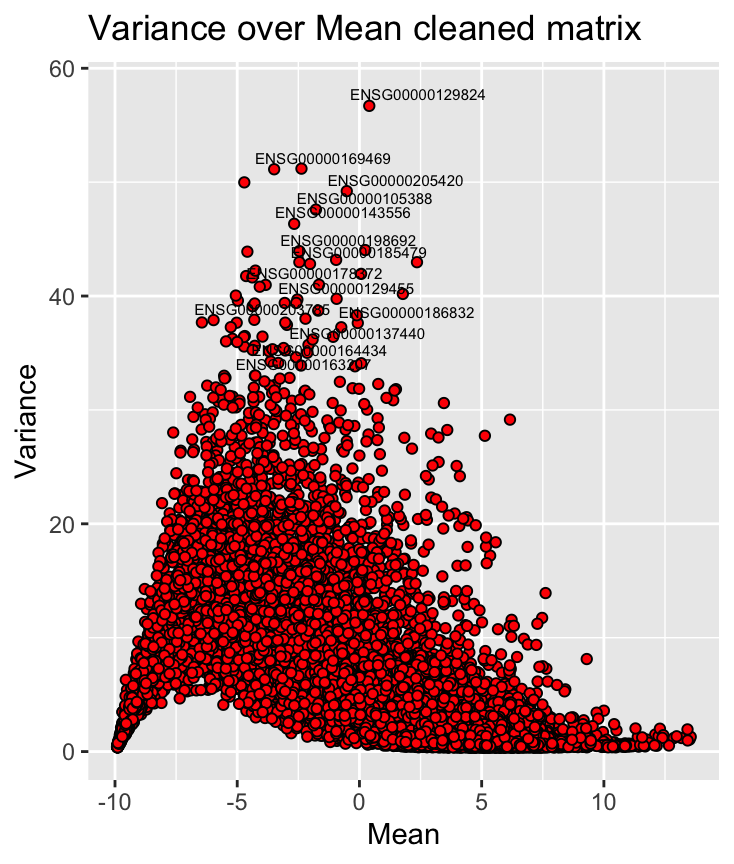
\includegraphics[width=0.3\linewidth]{figures/Variance_over mean_cleaned_matrix} 

}

\caption{Mean-variance plot of cleaned TCGA expression data. Y-axis shows variance of a genes expression, x-axis shows mean of a genes expression}\label{fig:showmeanvariance}
\end{figure}

\hypertarget{violin-plots}{%
\subsubsection{Violin Plots}\label{violin-plots}}

For descriptive analysis 5 violin plots were created for 5 different
tumor types with the gene expression data from the TCGA Matrix, to
compare the distribution of the data of 5 different tumor types. The
violinplot can be seen in Figure @ref(fig:showviolinplots). The white
point in the middle of each plot shows the 50\% quantile. For all tumor
types it is located in the middle of the gene expression value 0 and 5.
In this area is also the highest amount of genes for every tumor type.
Going to the top or bottom the curve flattens because only a few genes
are expression very high or very low. One can see, that the the
distributions of all 5 tumor types are very similar. It can be
concluded, that the other 28 tumor types of this data set are
distributed in a similar way.

\begin{figure}

{\centering 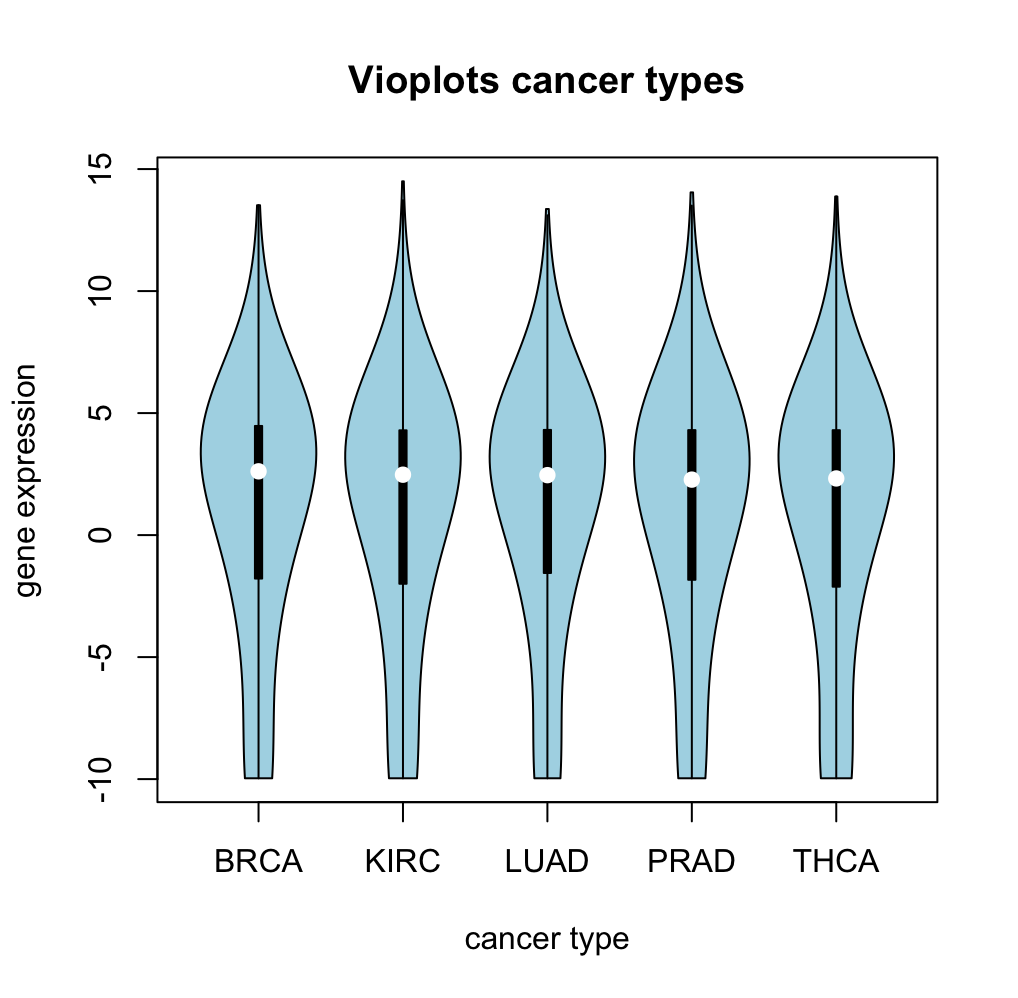
\includegraphics[width=0.3\linewidth]{figures/Vioplots cancer types} 

}

\caption{Mean-variance plot of cleaned TCGA expression data}\label{fig:showviolinplots}
\end{figure}

\hypertarget{volcano-plot}{%
\subsubsection{Volcano plot}\label{volcano-plot}}

For the construction of the volcano plot the data for THCA from the data
set for the focused analysis was used. The volcano plot is displayed in
Figure @ref(fig:showvolcanoplot). Not significantly differentially
expressed genes were marked green, significantly over expressed genes
are marked blue and significantly under expressed genes are marked red.
The gene with a very low p-value differ the most from tumor to normal
tissue and are annotated with their name.

\begin{figure}

{\centering 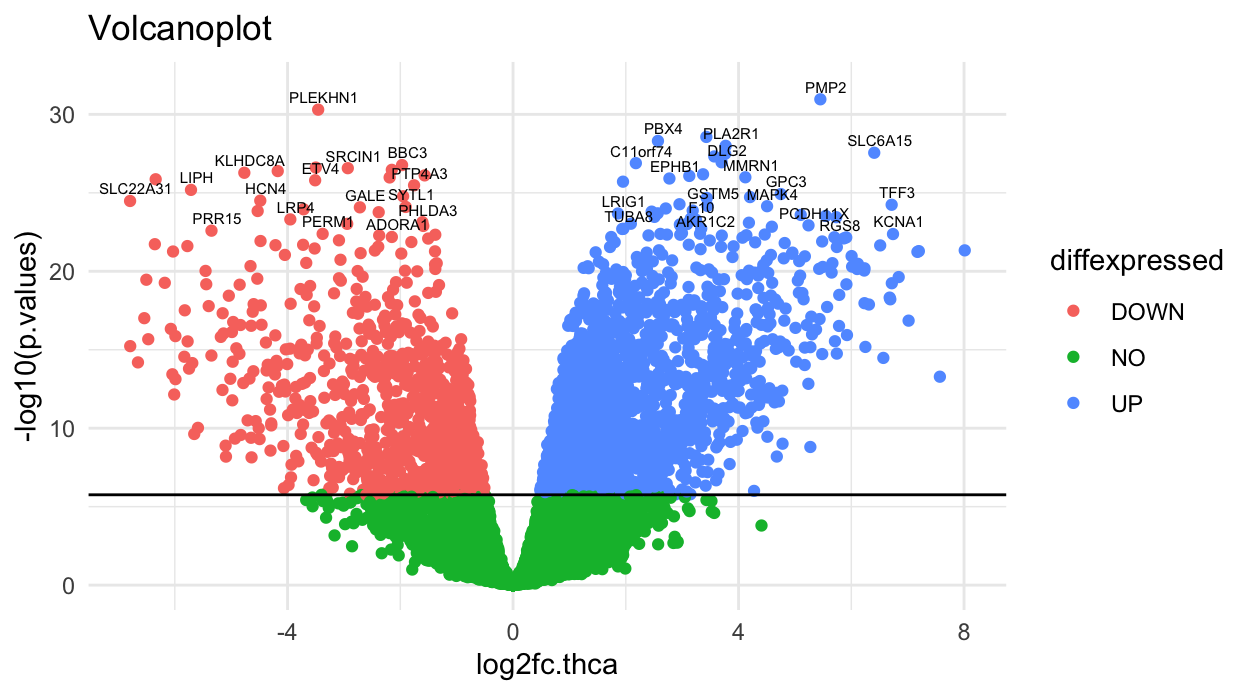
\includegraphics[width=0.3\linewidth]{figures/Volcanoplot} 

}

\caption{Volcano plot of THCA expression data}\label{fig:showvolcanoplot}
\end{figure}

\hypertarget{gsea}{%
\subsubsection{GSEA}\label{gsea}}

The results of the GSEA for THCA tissue can be seen in Figure
@ref(fig:GSEAHeat)

\begin{figure}

{\centering 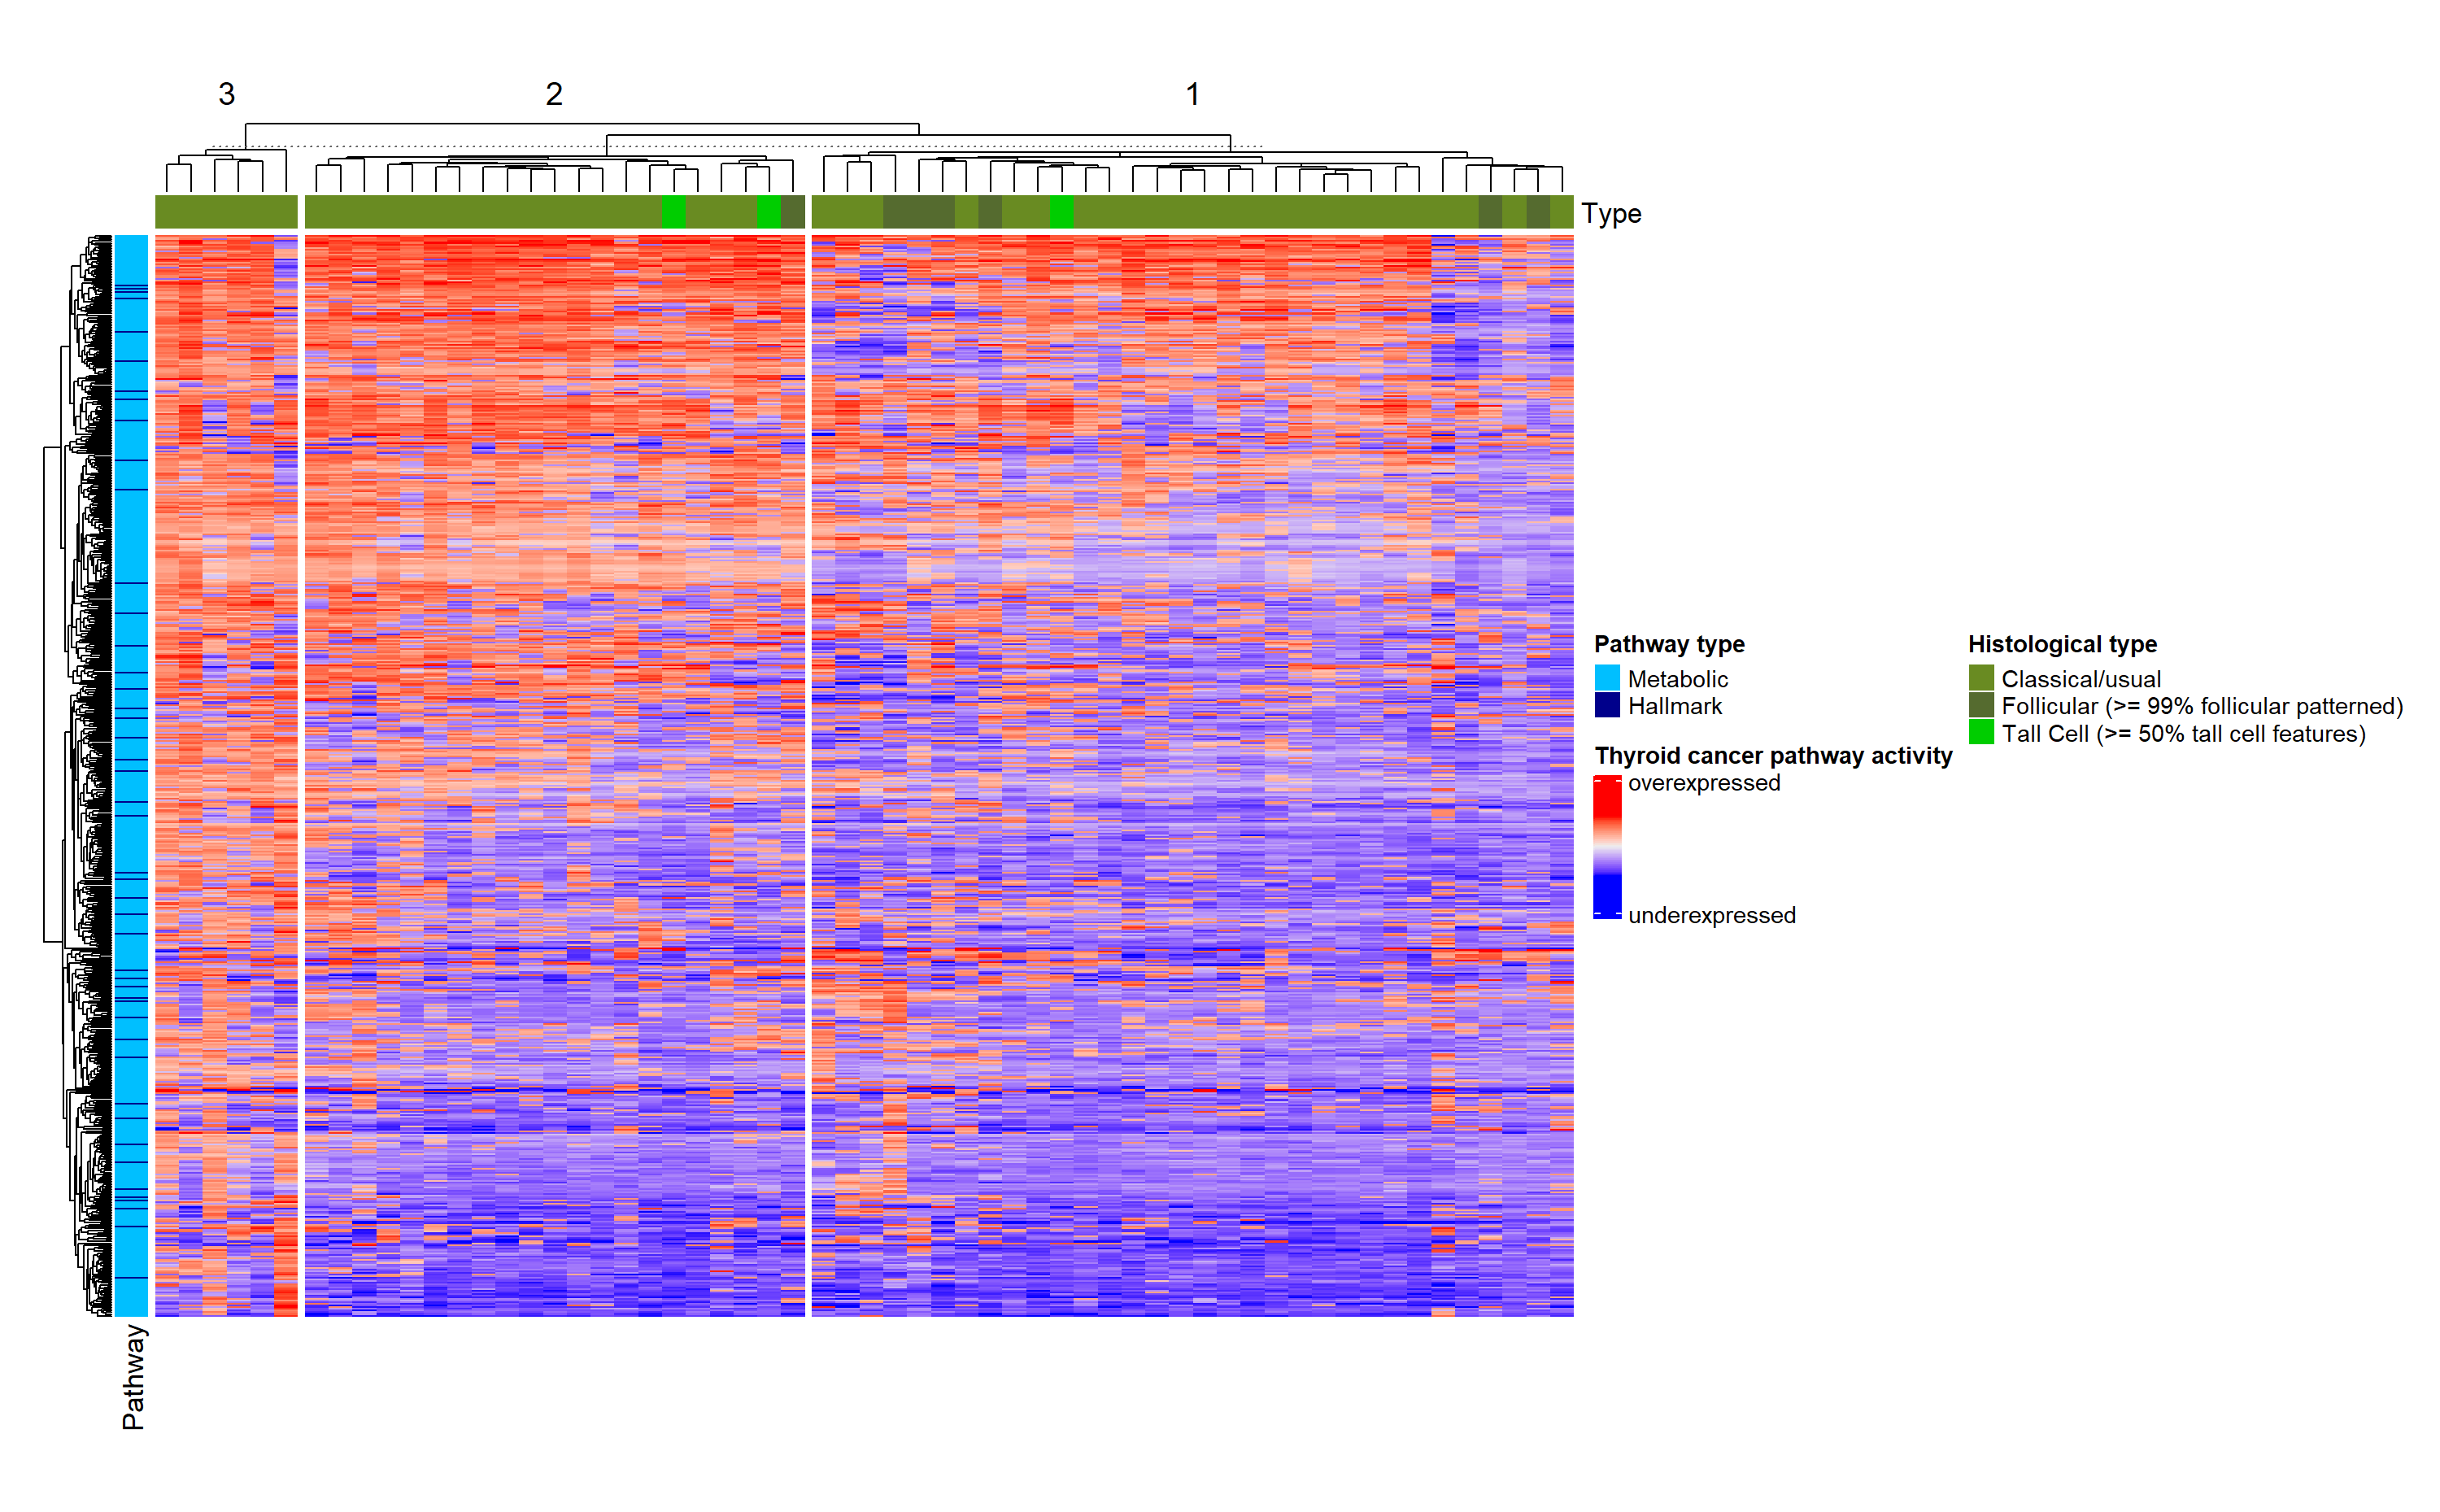
\includegraphics[width=0.9\linewidth]{figures/THCA GSEA Heatmap fertig} 

}

\caption{GSEA performed on the THCA expression data, annotated with Pathway type, histoligical type and cluster.}\label{fig:GSEAHeat}
\end{figure}

The patients are arranged horizontally, the pathways vertically. The
heatmap shows the intensity of expression of each pathway in each
patient. Red pathways are overexpressed, blue pathways are
underexpressed. The axes were annotated with the pathways type (hallmark
or metabolic), the histological type of the tumor and the cluster. Three
main clusters form within the patients, that can be explained by
similarities in pathway activity. It is possible, that the formation of
clusters is caused by different pathways activity of each tumor type,
because in cluster 3, only the classical type occurs, while tall cell
thyroid cancer mainly occur in cluster 2 and folicular thyroid cancers
mainly occur in cluster 1.

\hypertarget{pan-cancer-fuxfcr-thca---jakob}{%
\subsection{!!! pan cancer für THCA -
Jakob}\label{pan-cancer-fuxfcr-thca---jakob}}

Um die Clusterbildung zu bestätigen wurde die gleiche Analyse für die
THCA daten aus dem großen gene expression dataframe durchgeführt. Auch
in dieser Analyse formten sich 3 Cluster, die in zum Teil auf die
hiytological types zurückzuführen sind. xxx

\hypertarget{gsva}{%
\subsubsection{GSVA}\label{gsva}}

To display the results of GSVA, obtained by analysis of metabolic and
hallmark pathways and their expression in the gene expression data
frame, a heat map, annotated with cancer type, histological type and
pathway type was created. Even though, the individual pathways are not
annotated, two observations were made, because it is possible to see
similarities in pathway activity within groups of patients and tumor
types. Firstly 3 clusters in THCA expression were detected to analyse
them further in the next steps. Secondly, most tumor types were
clustered clearly, while others did not see to form explicit clusters
regarding the tumor type, but regarding the histological type. An
observation, that is going to be analysed further.

\begin{figure}

{\centering 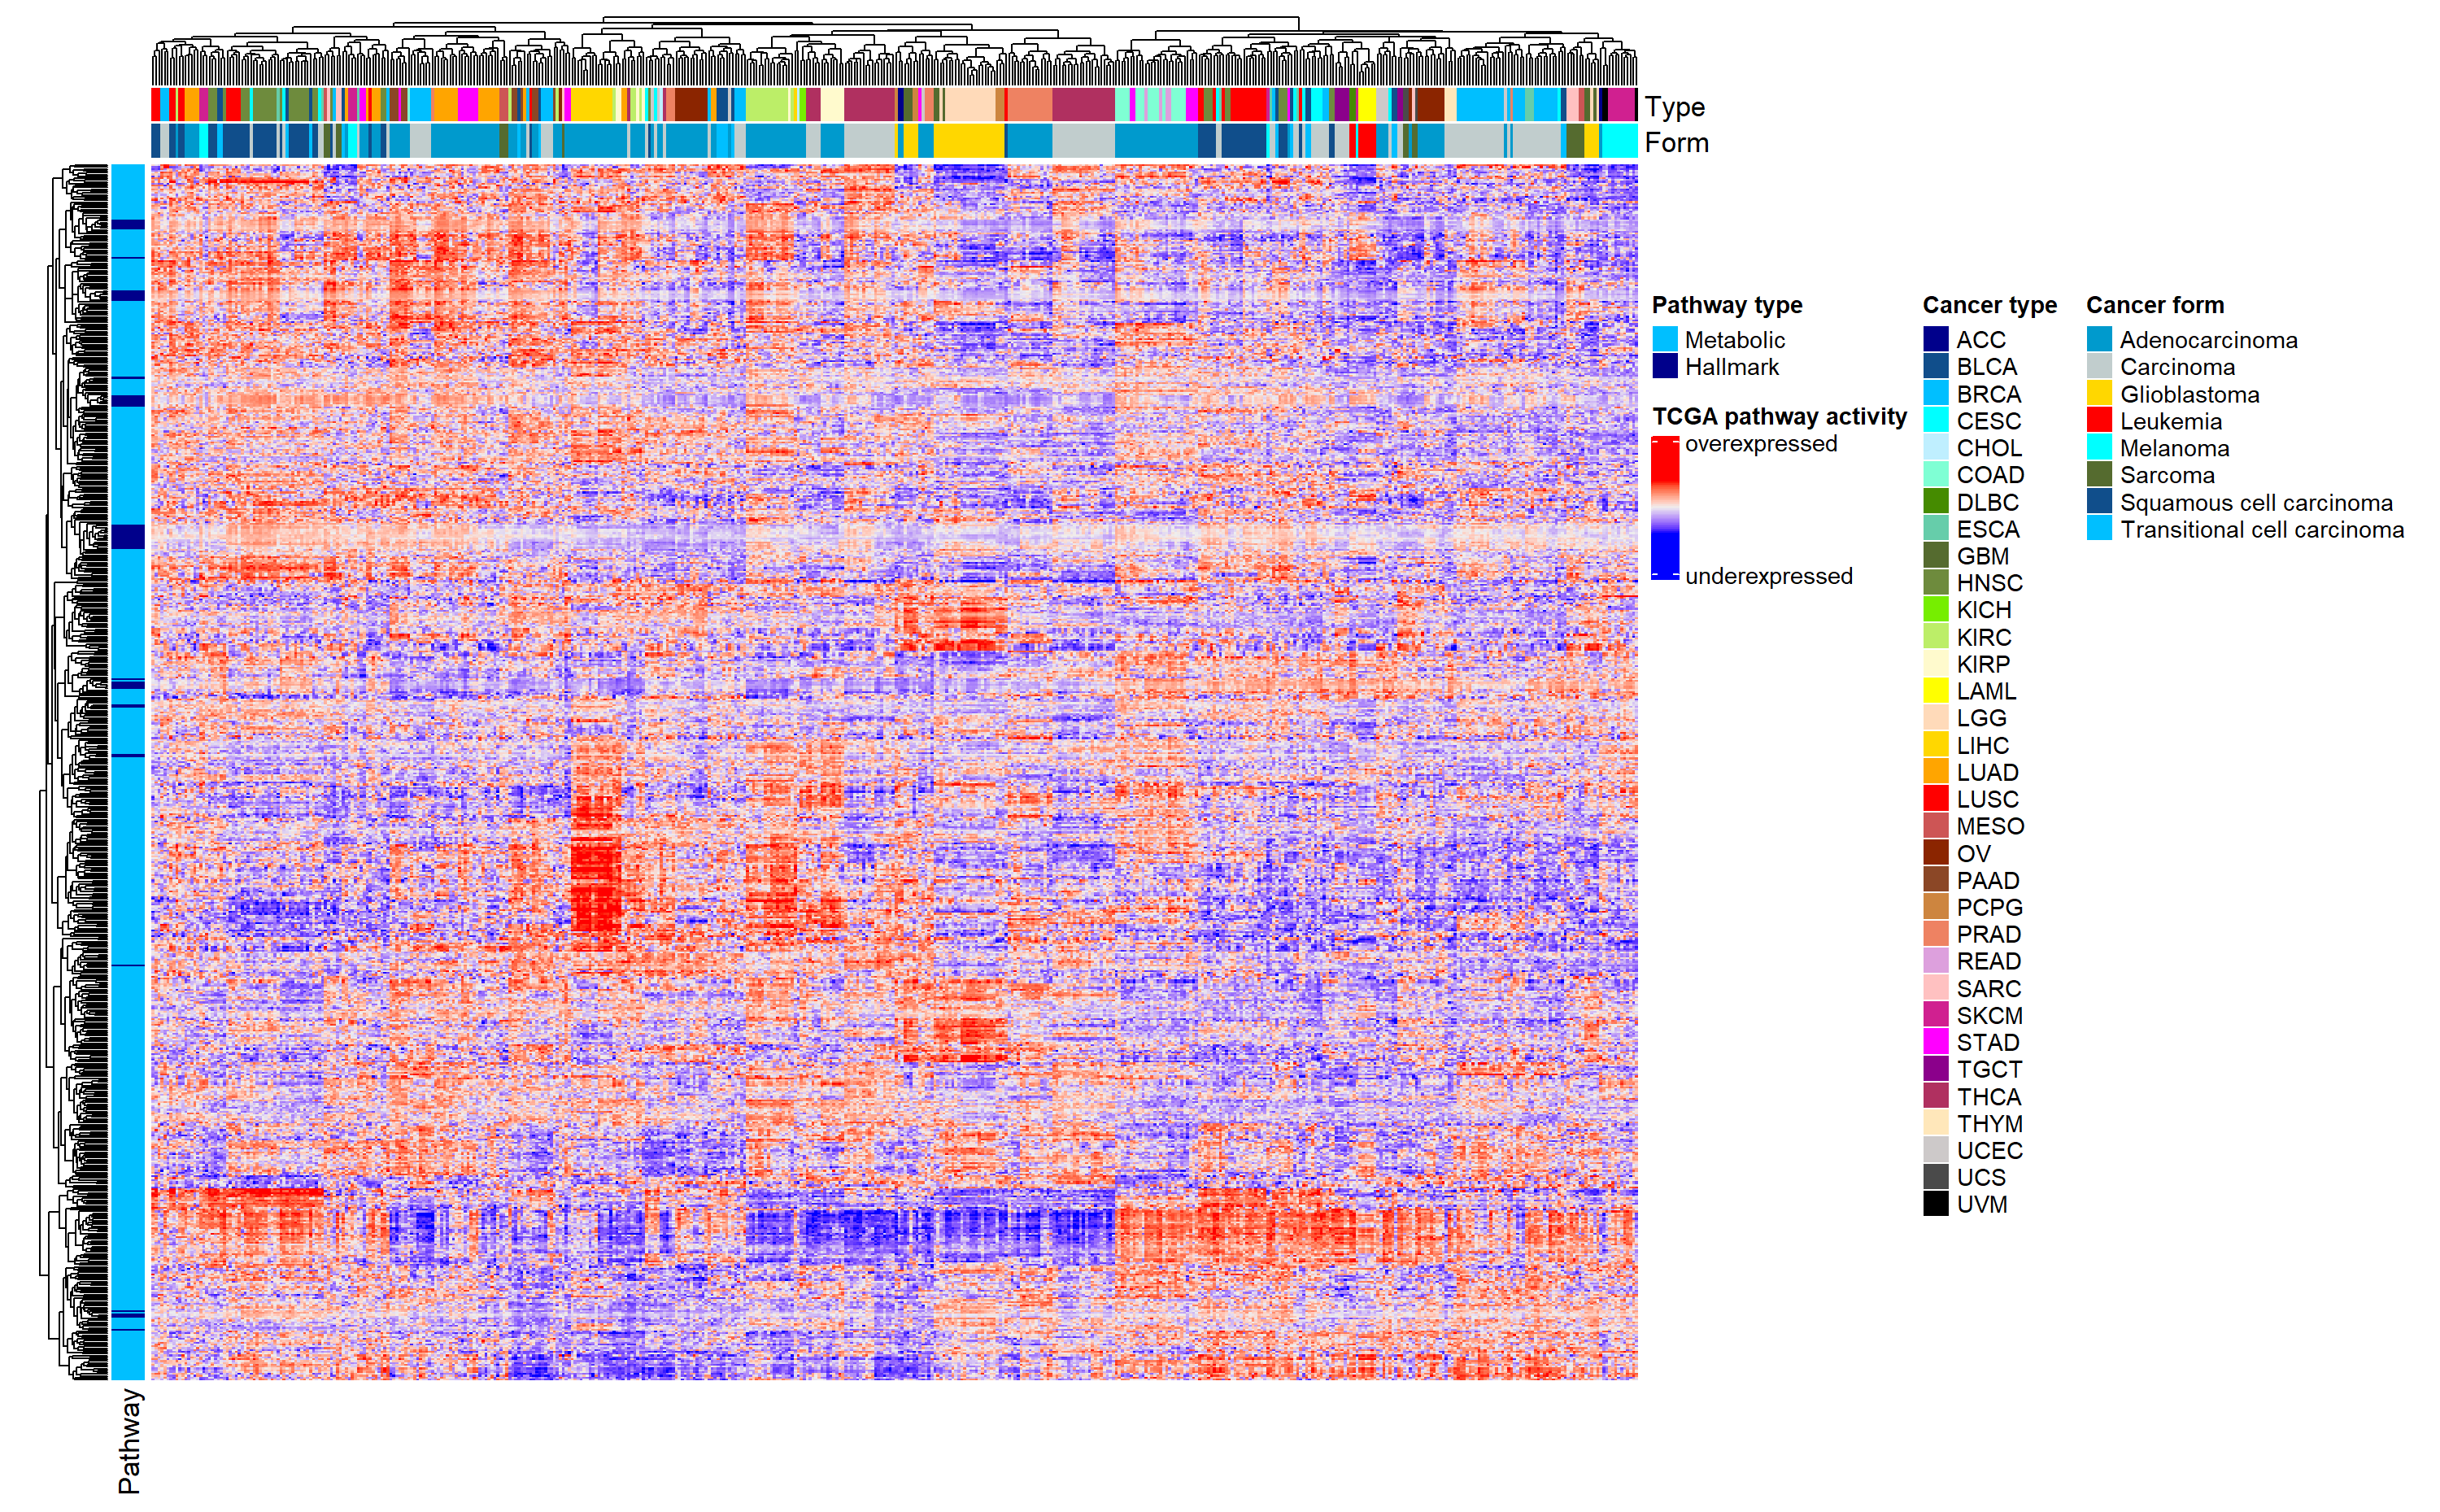
\includegraphics[width=1\linewidth]{figures/GSVA Heatmap fertig} 

}

\caption{Results of GSVA, annotated with histological type, cancer type, pathway type and clusters}\label{fig:GSVAHeat}
\end{figure}

The observations, obtained from GSVA and the generated heatmap were
checked with a heat map, displaying the mean expression of each pathway
in each tumor type, annotated with histological type and pathway type.
The tumor types were clustered based on their mean pathway activity. The
results confirm the formation of clusters based on the histological
type, therefore gene expression pattern is not dependent from each
individual or their tumor type but by the histological type. Another
observation is, that, the hallmark genes are mostly marked in a lighter
colour.

\begin{figure}

{\centering 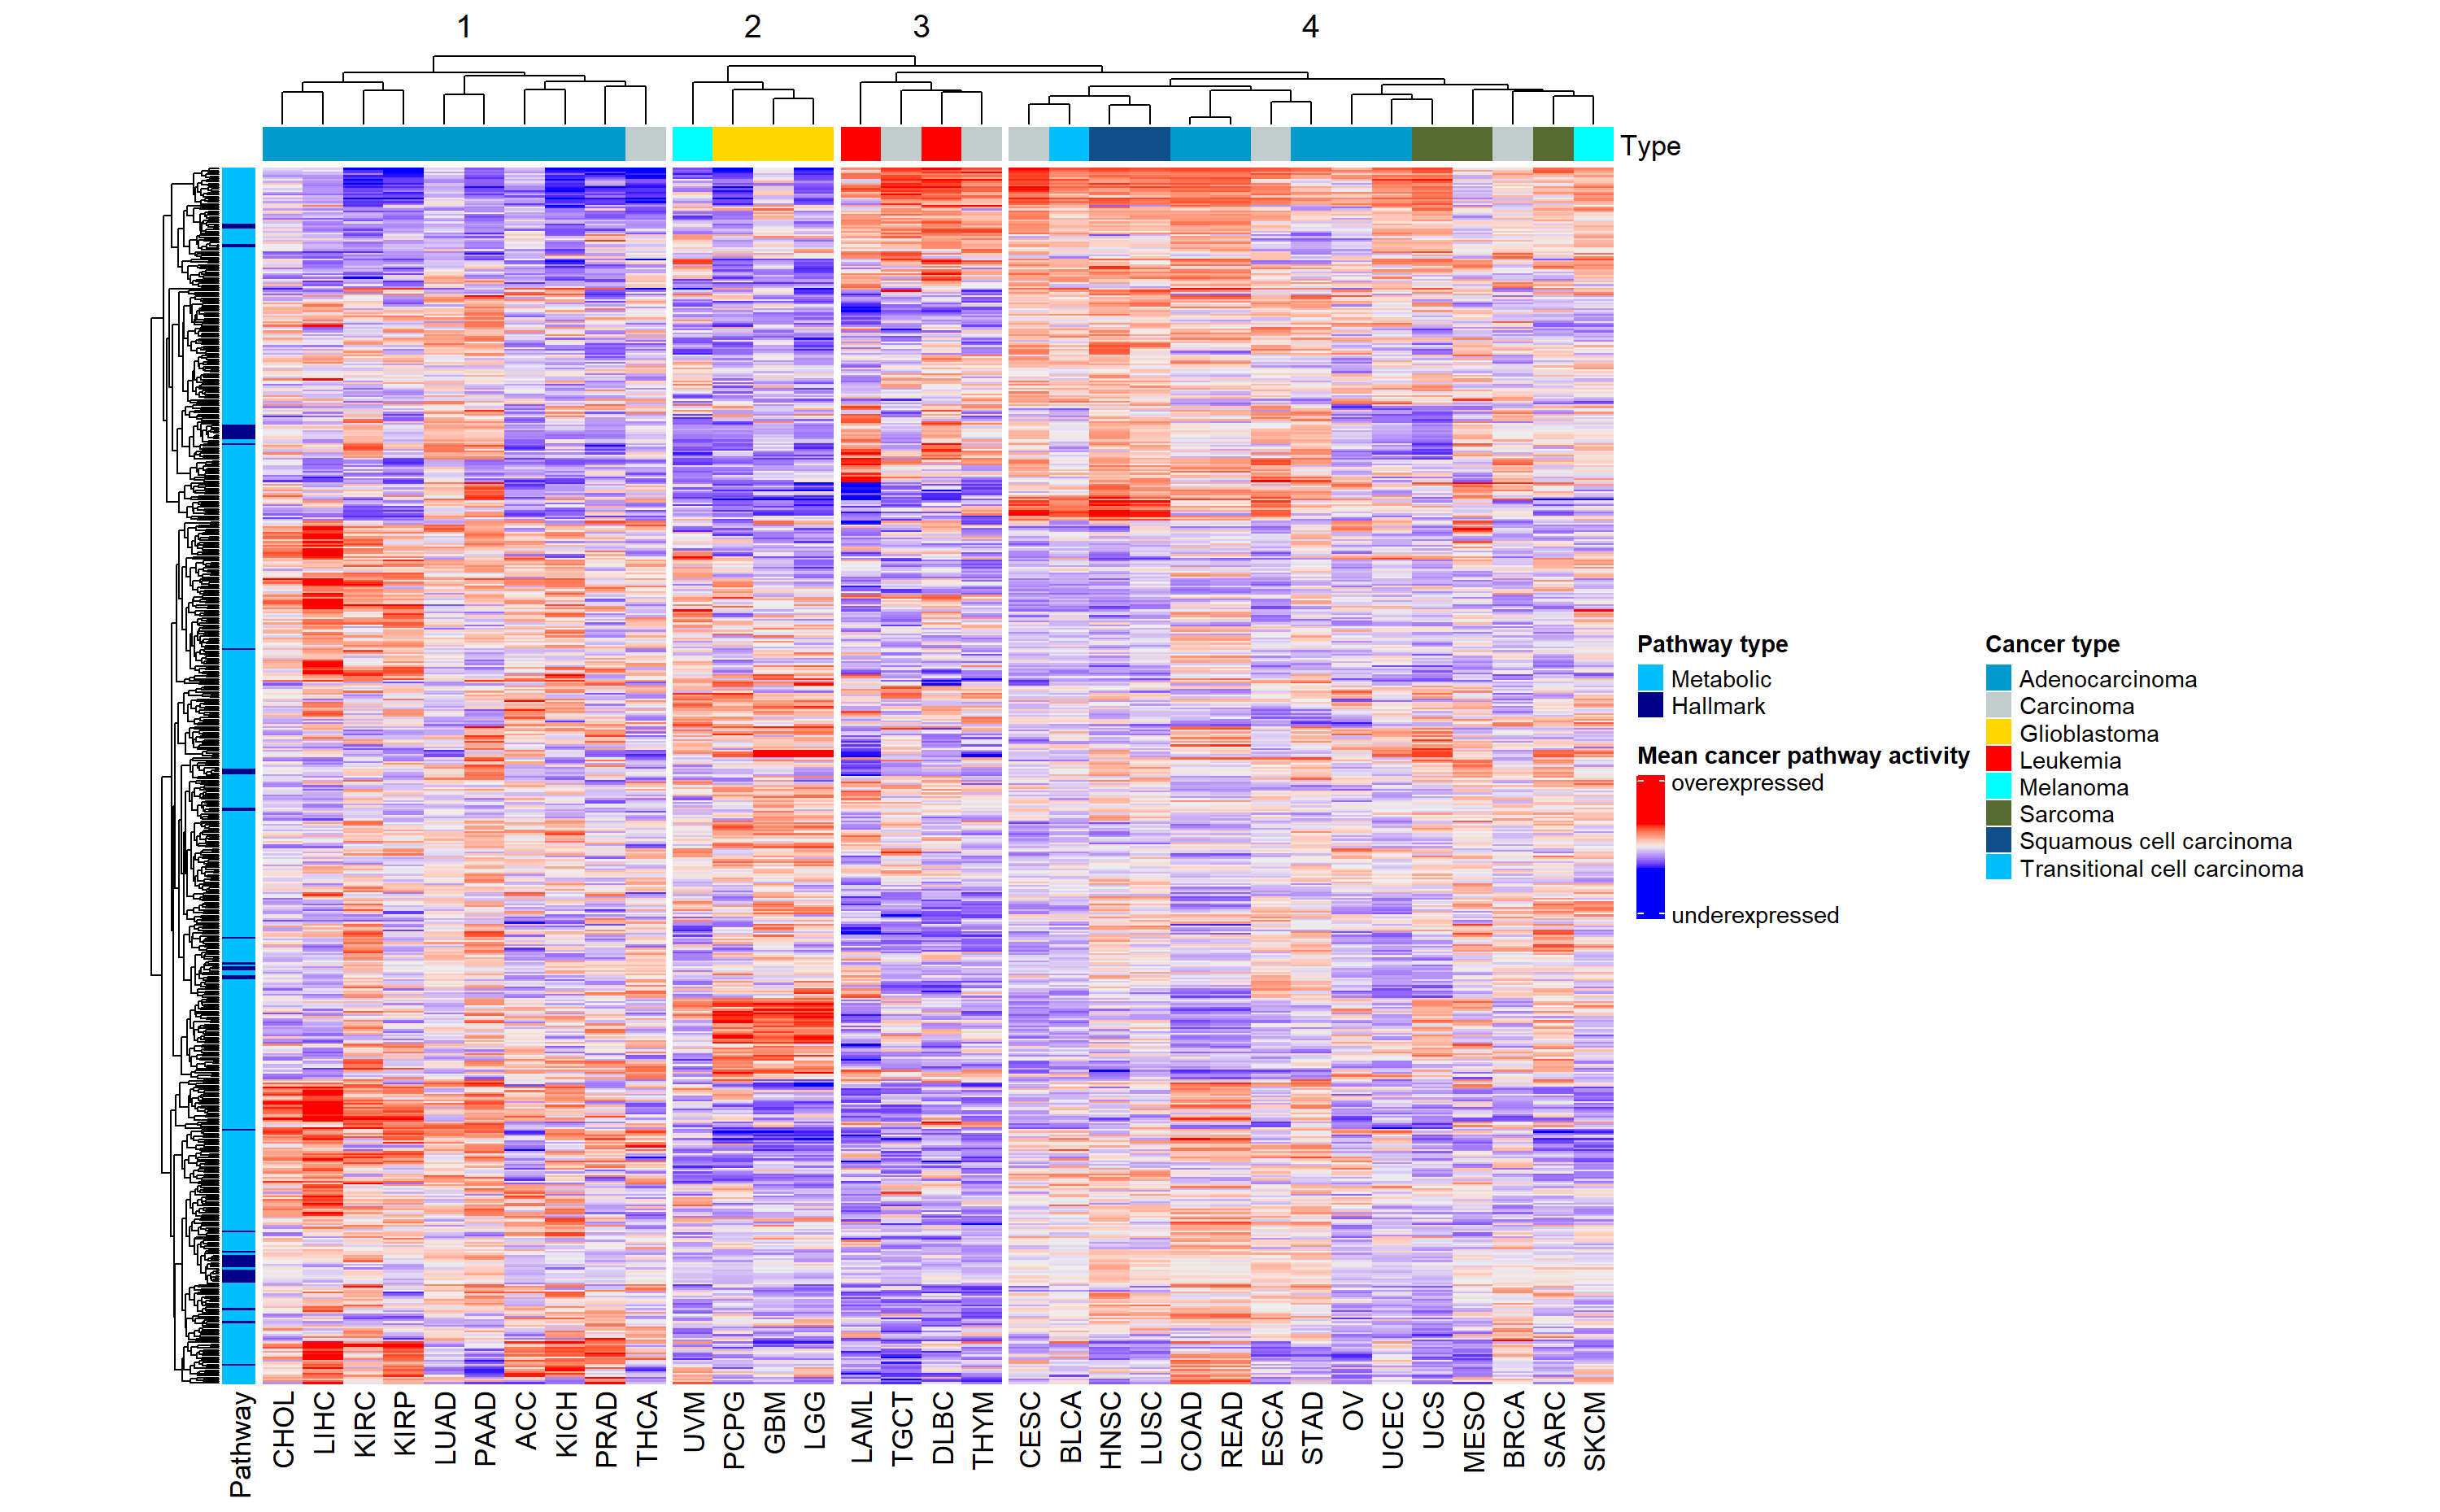
\includegraphics[width=0.5\linewidth]{figures/Pan Cancer mean expression} 

}

\caption{Mean expression of each pathway in each tumot type, annotated with pathway type, histological cancer type and clusters.}\label{fig:meanexp}
\end{figure}

\hypertarget{pca}{%
\subsubsection{PCA}\label{pca}}

The PCA was performed with the basis of the calculated pathway
activities and displayed in Figure @ref(fig:PCAPanType), reduced to the
first 2 PCs. Even though, clusters were formed in the analysis, they can
not be clearly identified, in the figure. The samples were parked by
tumor type and all patients of one tumor type occur in the same region,
but they do not form individual clusters. The same plot was colored by
histological type, showing, that patients with the same histological
type occur close to each other. The results from the PCA confirm the
results from the GSVA, pathways, that are included in th first two PCs,
seem to cohere with the histological type.

\begin{figure}

{\centering 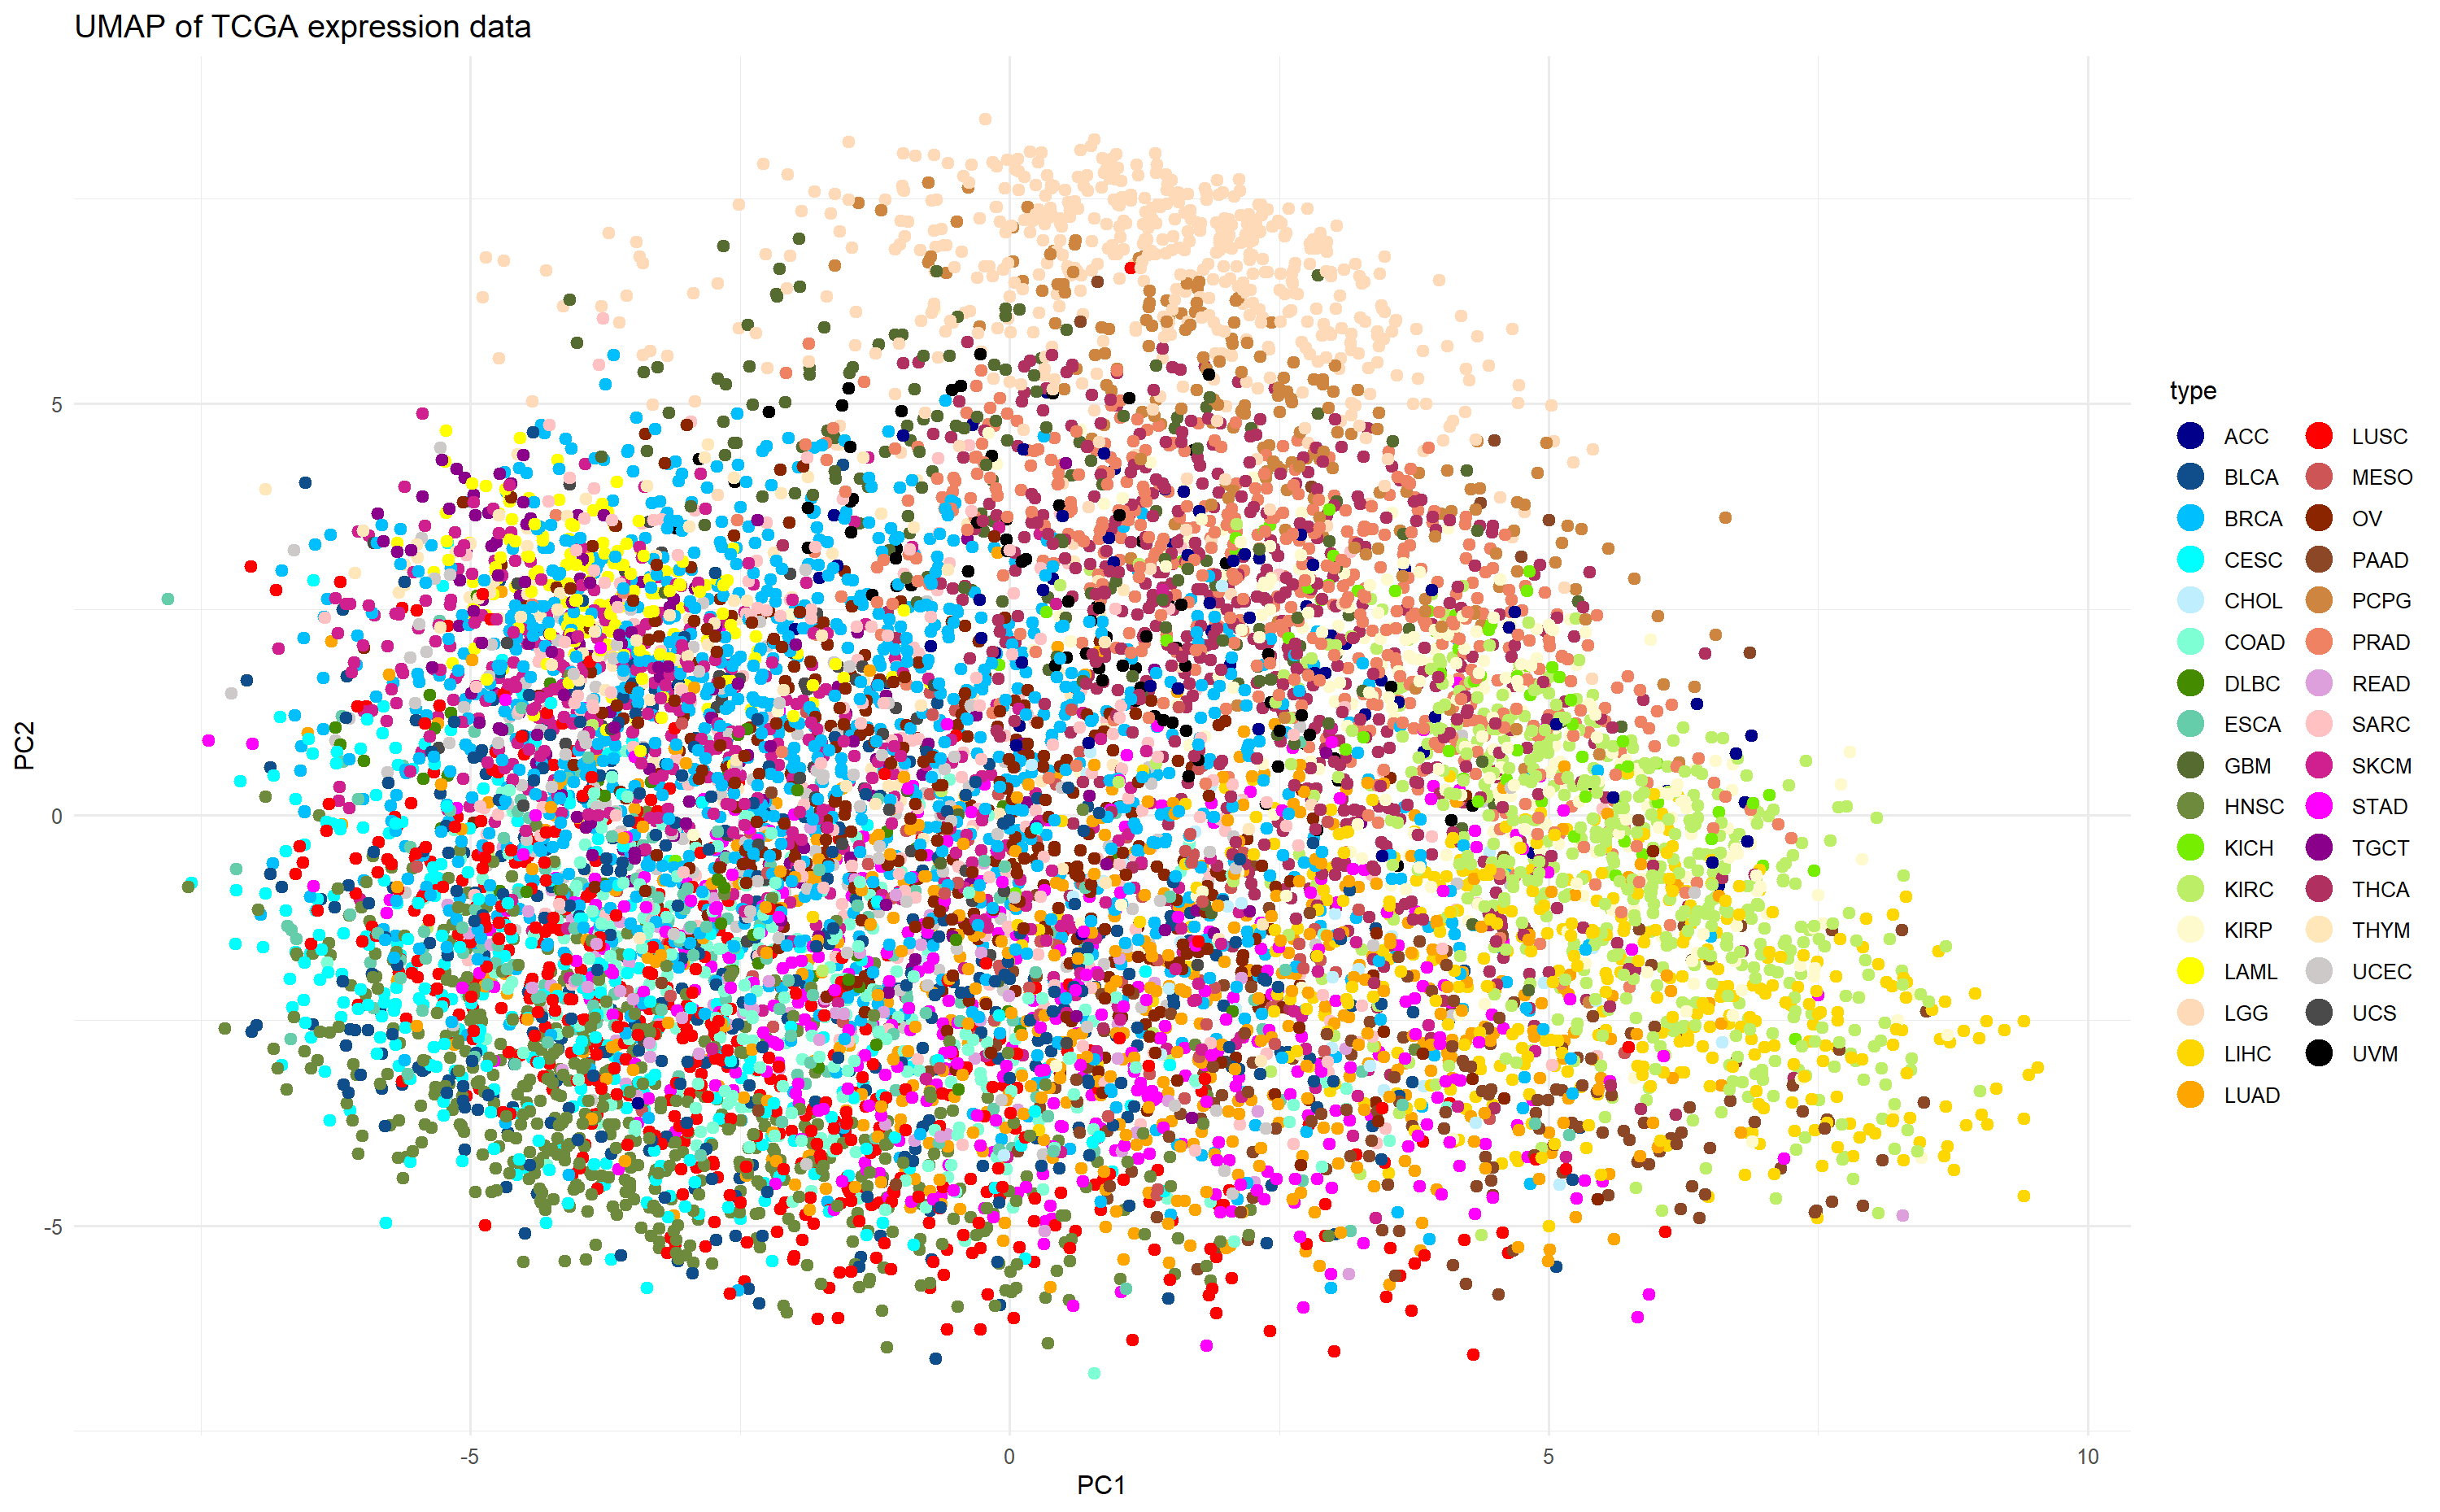
\includegraphics[width=0.75\linewidth]{figures/Pan Cancer PCA PC1und2} 

}

\caption{PCA of TCGA expression data, colored by tumor type}\label{fig:PCAPanType}
\end{figure}

\begin{figure}

{\centering 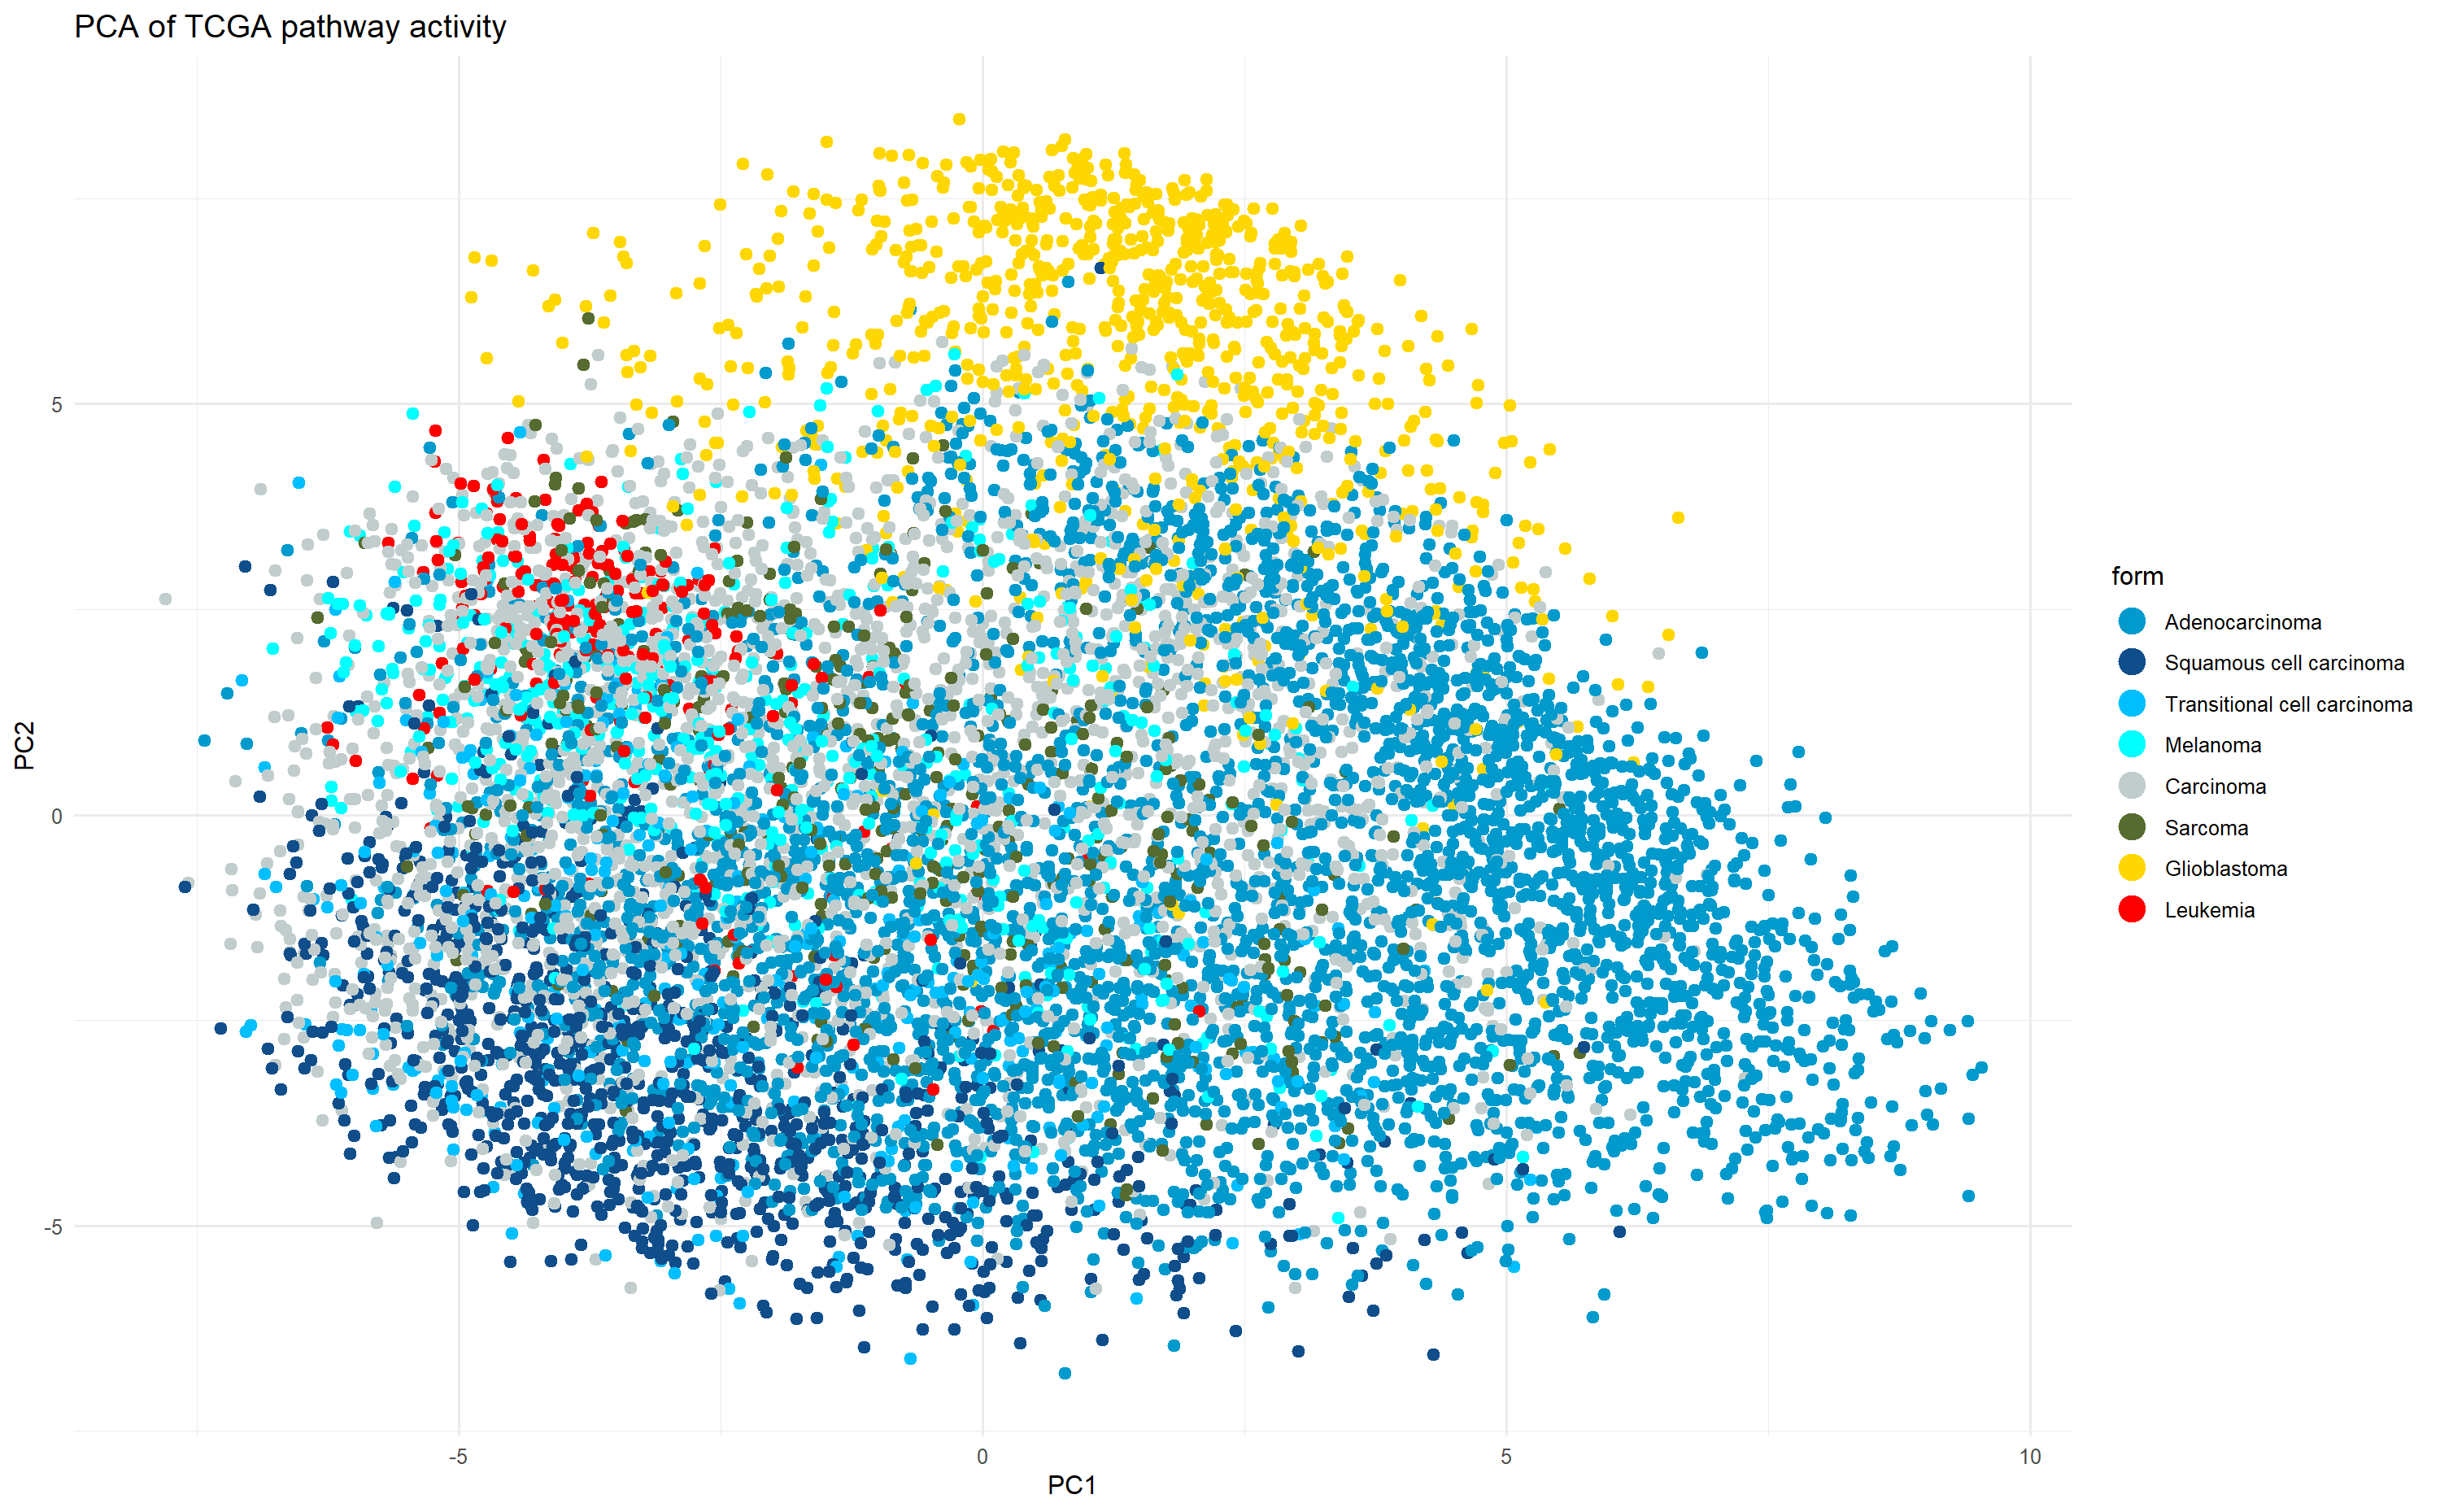
\includegraphics[width=0.75\linewidth]{figures/Pan Cancer PCA PC1und2 cancer form} 

}

\caption{PCA of TCGA expression data, colored by form of tumor}\label{fig:PCAPanForm}
\end{figure}

\hypertarget{umap}{%
\subsubsection{UMAP}\label{umap}}

Because the cluster structure displayed by the PCA was not as expected,
the results from the PCA were used to create a UMAP. In Figure
@ref(fig:UMAPPanType) clear clusters can be seen, what reassures, that
the tumor types have characteristic pathway activities. In the middle a
big cluster can be seen, that can not be assigned to a certain tumor
type. To detect the cause for this cluster, the UMAP was colored by
histological types (Figure @ref(fig:UMAPPanForm)), showing, that the big
cluster in the middle mainly contains various carcinoma types like
squamous cell carcinoma and transitional cell carcinoma. The UMAP
confirmed again the assumption, that the histological type of a tumor
has a mayor impact on the patients gene expression profile.

\begin{figure}

{\centering 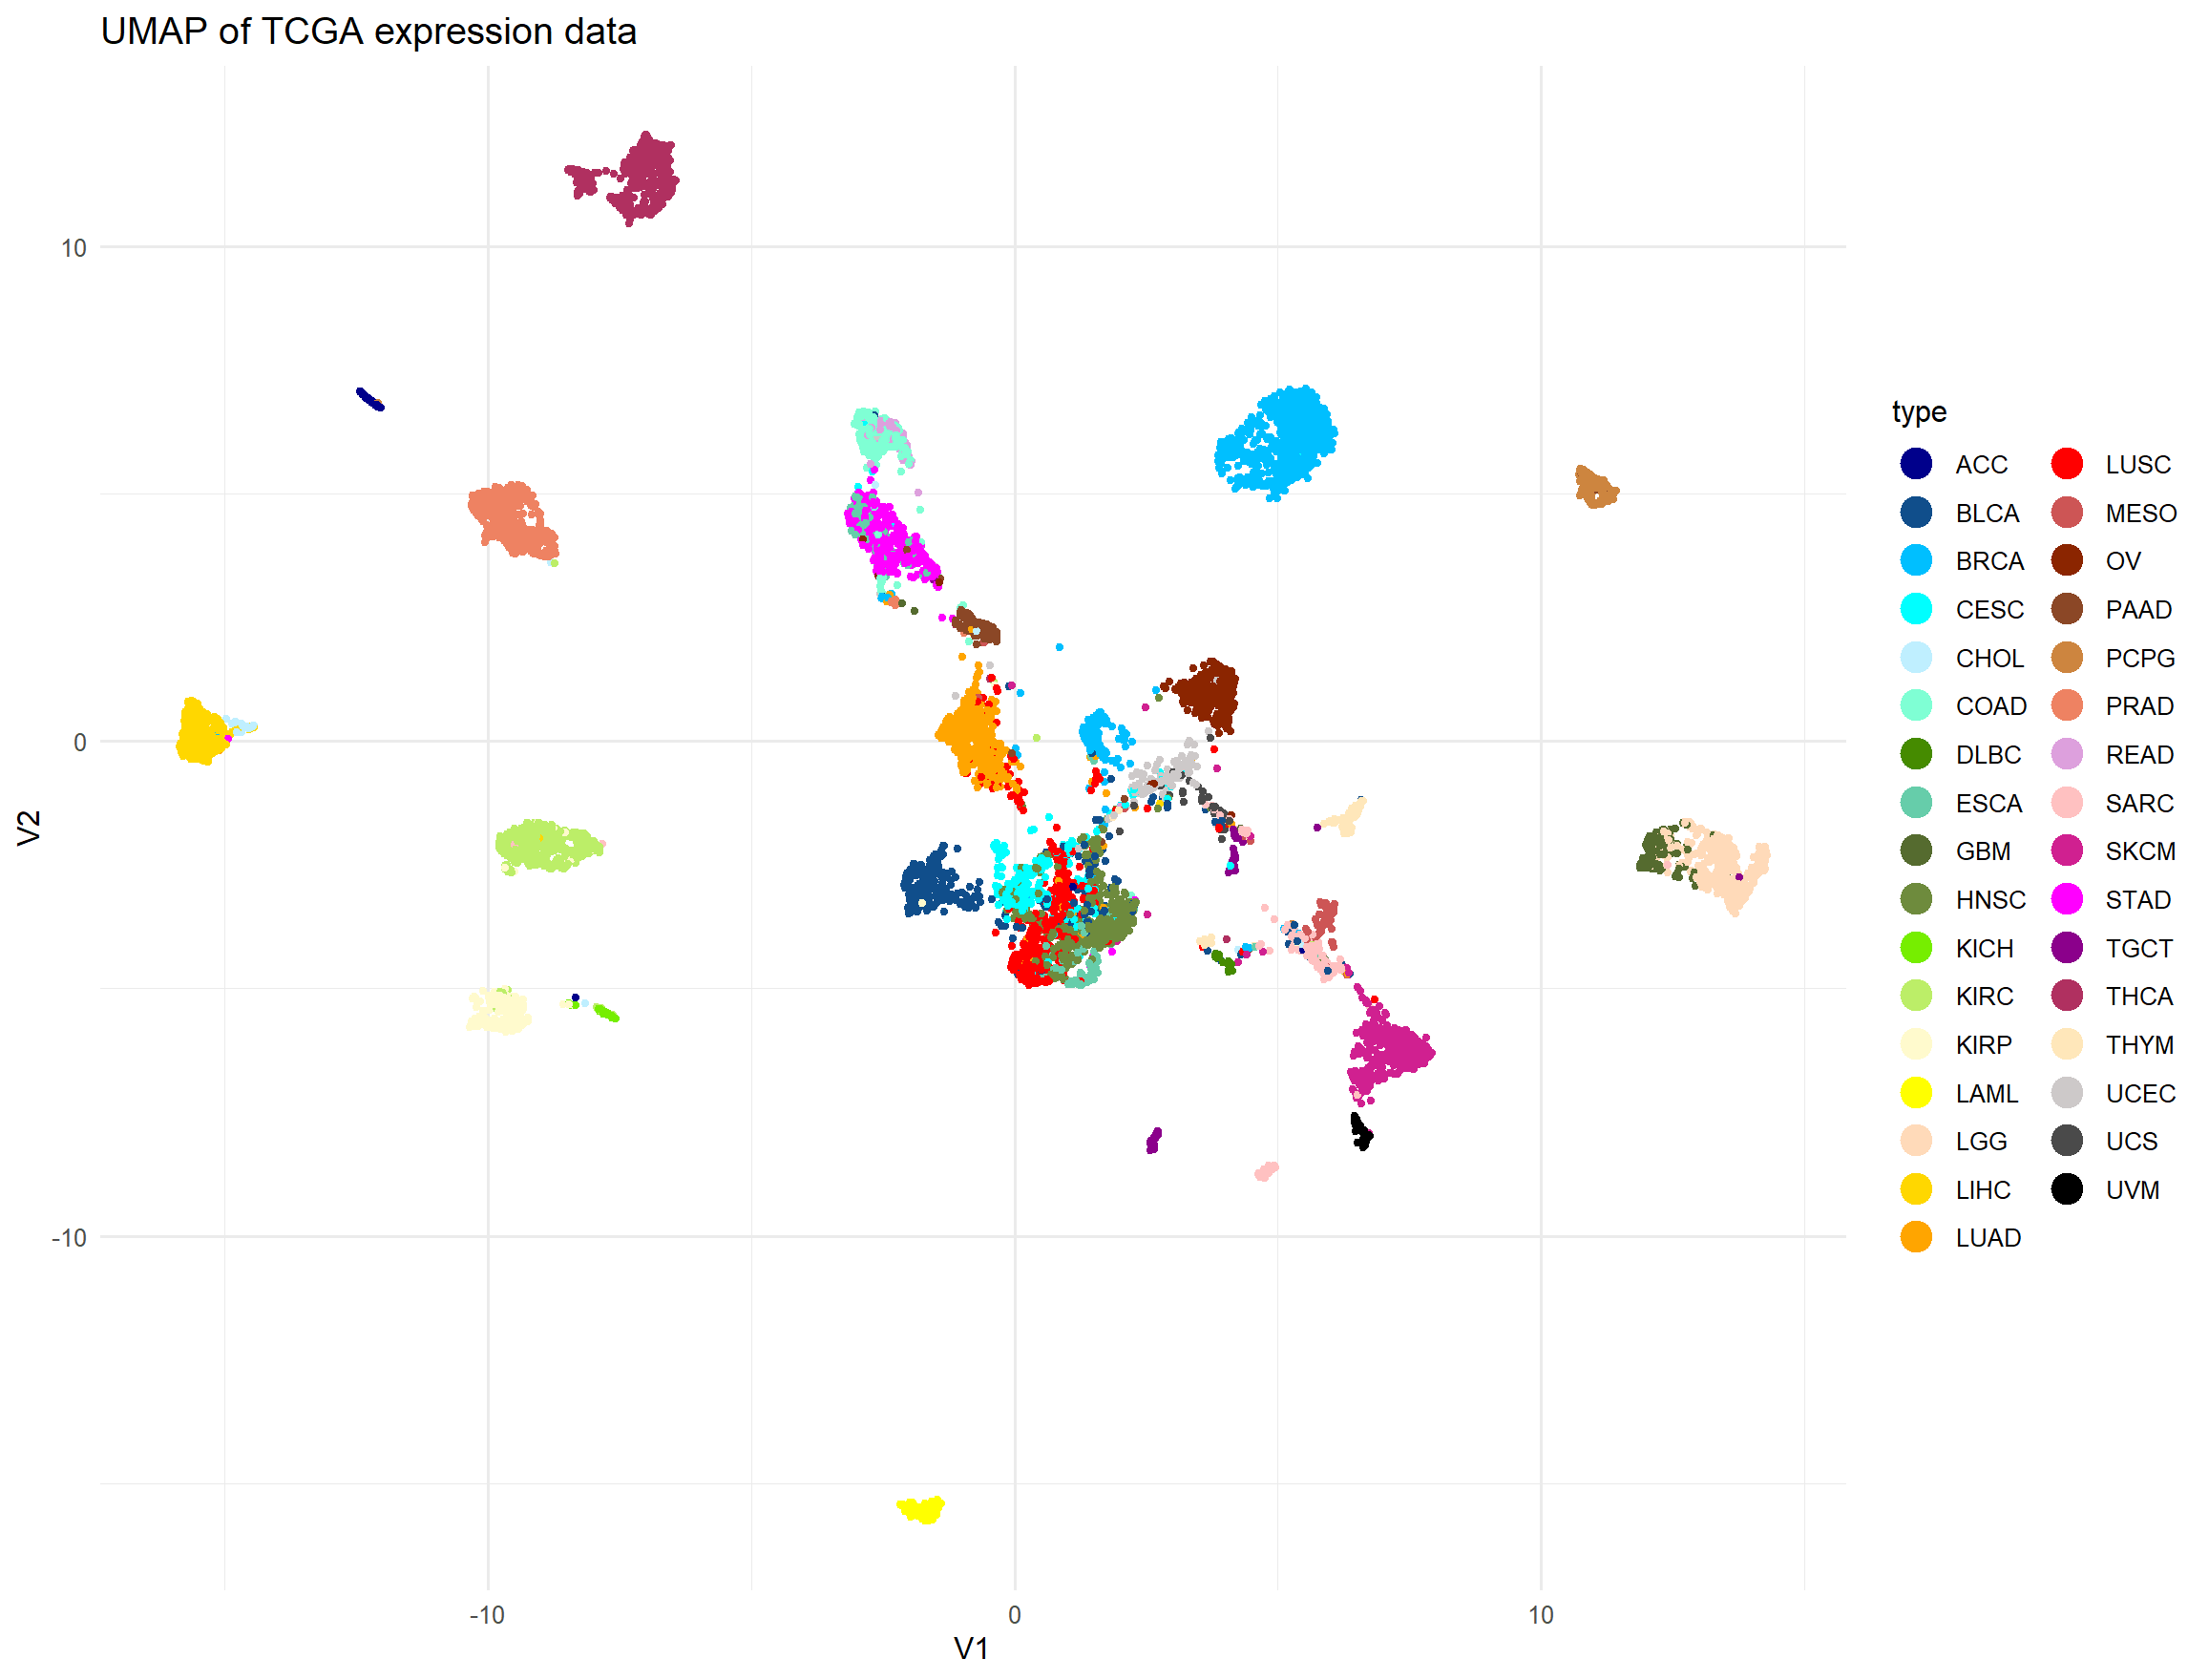
\includegraphics[width=0.5\linewidth]{figures/Pan Cancer UMAP} 

}

\caption{UMAP of TCGA expression data, colored by tumor type}\label{fig:UMAPPanType}
\end{figure}

\begin{figure}

{\centering 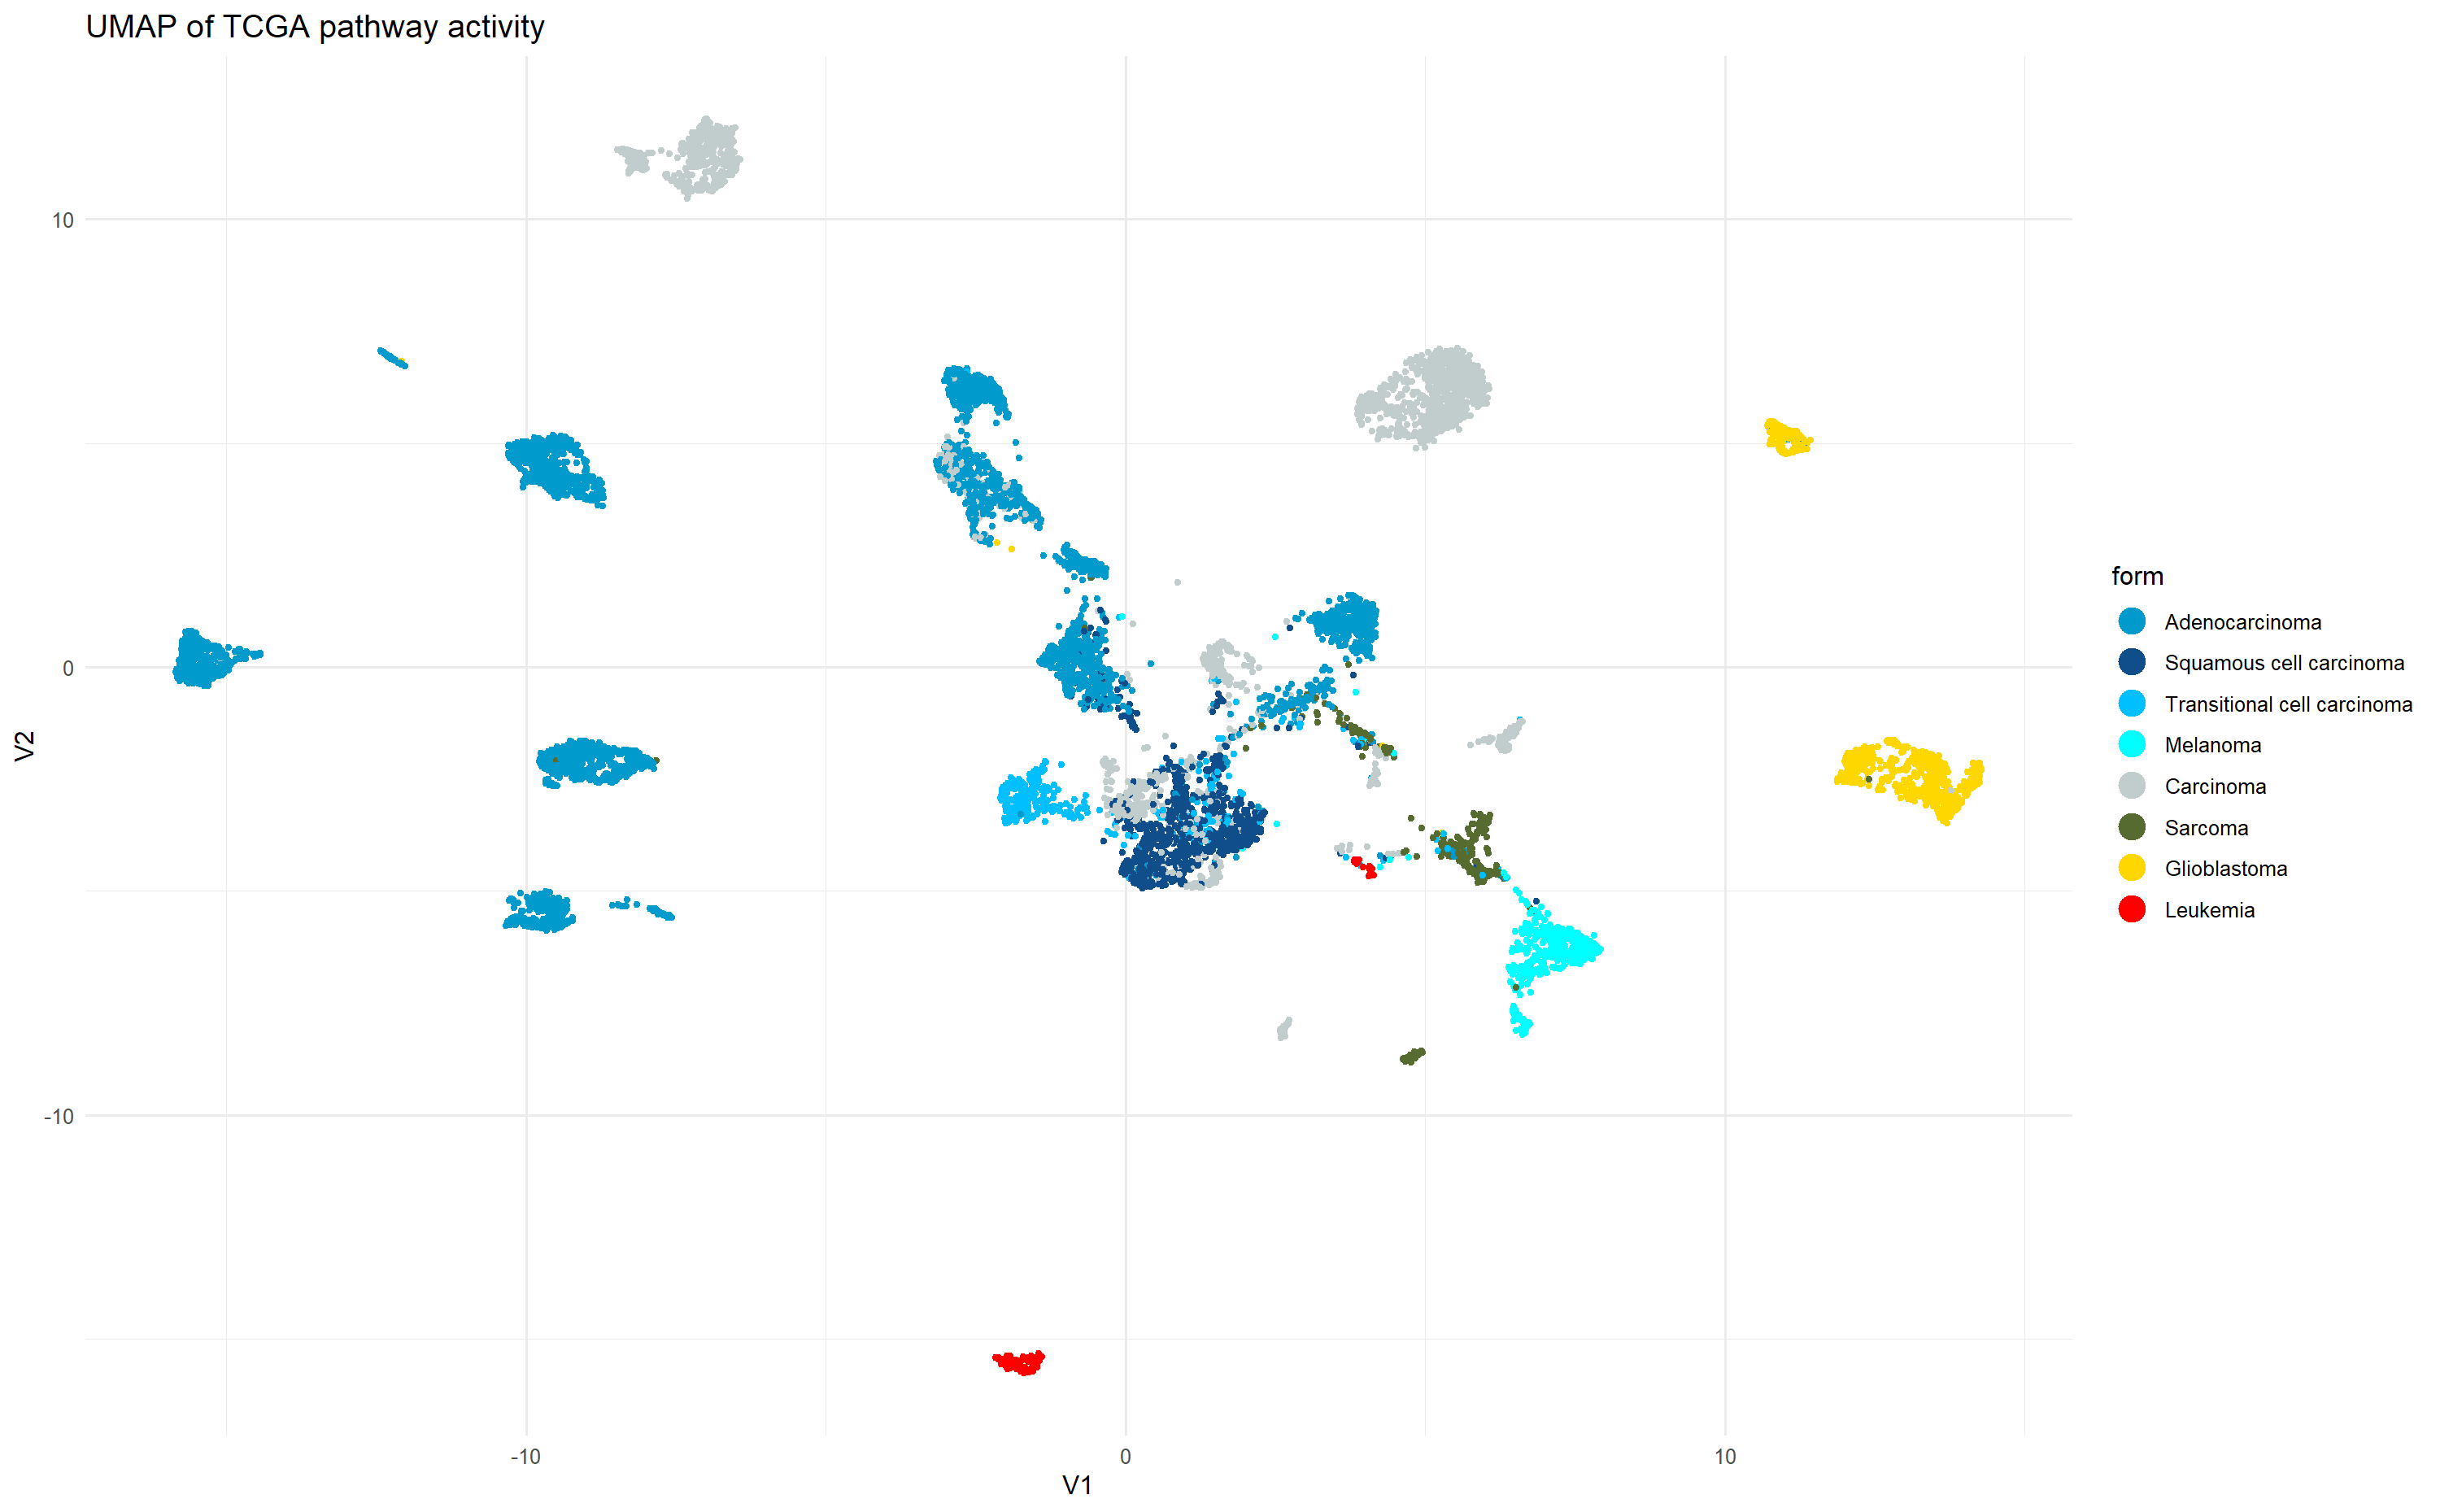
\includegraphics[width=0.5\linewidth]{figures/Pan Cancer UMAP cancer form} 

}

\caption{UMAP of TCGA expression data, colored by form of the tumor}\label{fig:UMAPPanForm}
\end{figure}

The same analysis was performed for gene activity instead of pathway
activity to check for reliability of the results. No differences could
be detected,

\hypertarget{regression-analysis}{%
\subsubsection{Regression analysis}\label{regression-analysis}}

\hypertarget{focused-analsis}{%
\subsubsection{Focused analsis}\label{focused-analsis}}

\hypertarget{pca-1}{%
\subsubsection{PCA}\label{pca-1}}

PCA was also performed for focused analysis, um Untergruppen, die mit
der Pathwayaktivität oder Genaktivität zusammenhängen, innerhalb der
Thyroid tumors zu finden. Dafür wurden zuerst die Ergebnisse der GSEA
verwendet. Der Versuch Cluster zu finden gestaltete sich hier leider
schwerer, da weder durch Betrachtung des Thyroid Tumortyps, noch durch
Betrachtung der Stage ein eindeutiger Zusammenhang erkannt werden
konnte.

\hypertarget{figure-x}{%
\subsubsection{Figure X}\label{figure-x}}

A figure x was generated for THCA gene expression data obtained from the
gene expression data frame. The obtained figure x can be seen in Figure
@ref(fig:figurex). Thereby pathways with the lowest p-value could be
identified. The pathway for thyroxine biosynthesis is a downregulated
pathway with a low p-value and is going to be predicted by linear
regression analysis and the neuronal network.

\begin{figure}

{\centering 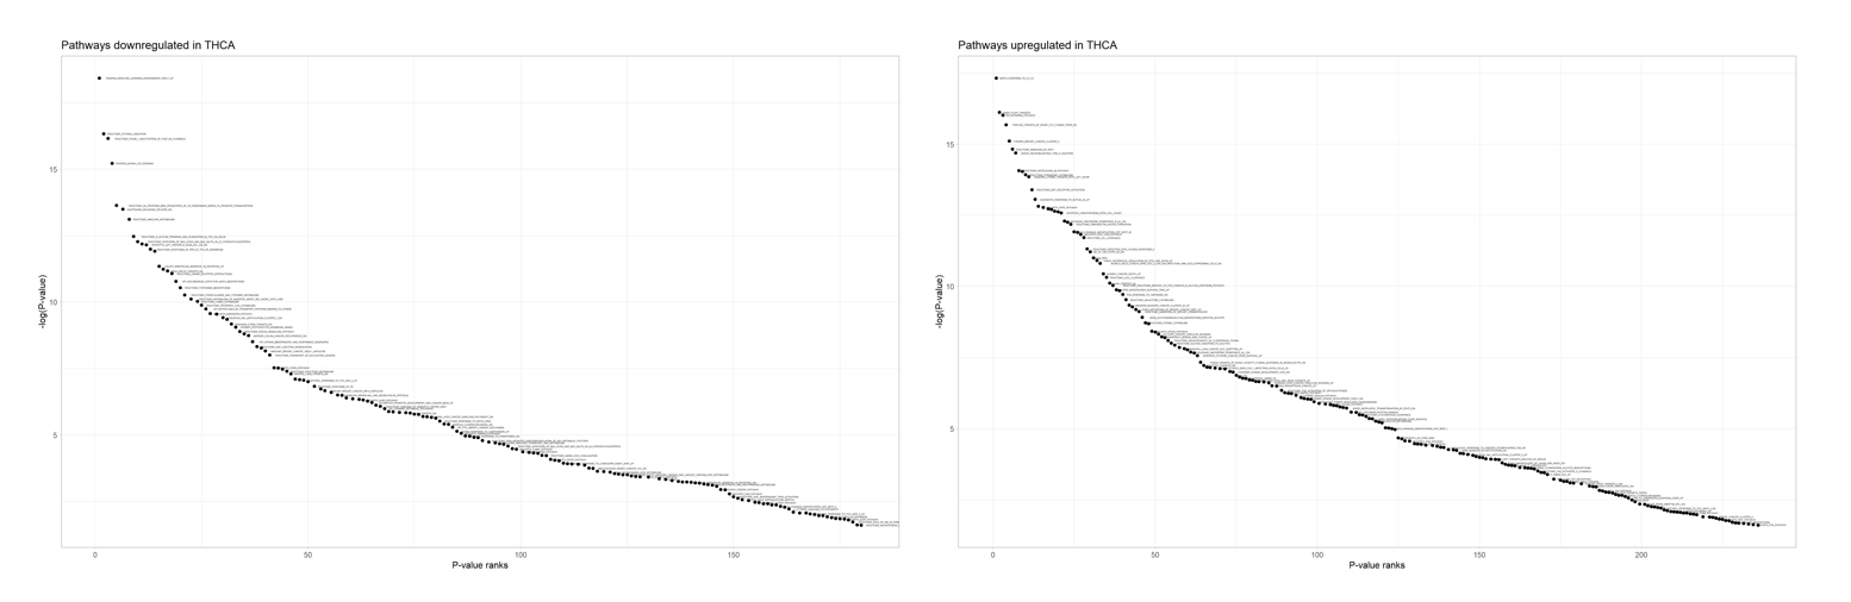
\includegraphics[width=1\linewidth]{figures/2figurexTHCA} 

}

\caption{Figure X. -log10(p-values) plotted against ranked p-values, obtained from GSVA on THCA expression data from gene expression data frame. Left: downregulated pathways, right: upregulated pathways}\label{fig:figurex}
\end{figure}

\begin{center}\rule{0.5\linewidth}{0.5pt}\end{center}

\hypertarget{discussion}{%
\chapter{Discussion}\label{discussion}}

In der PCA war vermutlich nicht so ein gutes ergebnis zu erkennen, weil
nur die ersten 2 PCs verwendet wurden und dadurch nicht die gesamte
Varianz erklärt wurde. Bei verwendung aller PCs in der UMAP waren
eindeutige Cluster zu erkennen.

Die Ergebnisse der UMAPs entsprechen der Erwartungen. Carcinomas haben
alle ähnliche Expressionsmuster, da sie alle epithelialen Zellen
entspringen und deshalb ähnliche Mechanismen brauchen, um zu einer
Tumorzelle zu werden. Die expressionsmuster zu anderen hiytological
tumor types unterscheiden sich. Das liegt daran, dass verschiedene
genetische Mechanismen zur Tumorentstehung führen.

GSVA mittlerer expressionswerte: dass hallmark pathways alle weiß sind
entspricht unseren erwartungen

Epigeentic profiles = auch epigenetische veränderungen werden in die
Expressionsdate mit inebezogen, das wäre sehr sinnvol für die ANalyse,
wird hier aber nicht beachetet

/ref\{RNAseq\} /ref\{histological\_types\} (Stark \emph{et al.}, 2019)
\# References

\hypertarget{refs}{}
\begin{CSLReferences}{0}{0}
\leavevmode\vadjust pre{\hypertarget{ref-kumar_multiple_2017}{}}%
Kumar, SK, Rajkumar, V, Kyle, RA, Duin, M van, Sonneveld, P, Mateos,
M-V, Gay, F, and Anderson, KC (2017). Multiple myeloma. Nat Rev Dis
Primers 3, 17046.

\leavevmode\vadjust pre{\hypertarget{ref-RNAseq}{}}%
Stark, R, Grzelak, M, and Hadfield, J (2019). RNA sequencing: The
teenage years. Nature Reviews Genetics 20, 631--656.

\end{CSLReferences}

\hypertarget{appendix}{%
\chapter{Appendix}\label{appendix}}

\hypertarget{plots}{%
\section{Plots}\label{plots}}

hello \#\# Code world

\begin{Shaded}
\begin{Highlighting}[]
\CommentTok{\#createn einer liste mit allen patienten in dfs sortiert nach krebs}
\NormalTok{cancers }\OtherTok{=} \FunctionTok{list}\NormalTok{();cancers }\OtherTok{=} \FunctionTok{vector}\NormalTok{(}\StringTok{\textquotesingle{}list\textquotesingle{}}\NormalTok{,}\FunctionTok{length}\NormalTok{(}\FunctionTok{table}\NormalTok{(tcga\_anno}\SpecialCharTok{$}\NormalTok{cancer\_type\_abbreviation)))}
\FunctionTok{names}\NormalTok{(cancers) }\OtherTok{=} \FunctionTok{names}\NormalTok{(}\FunctionTok{table}\NormalTok{(tcga\_anno}\SpecialCharTok{$}\NormalTok{cancer\_type\_abbreviation))}
\NormalTok{i}\OtherTok{=}\DecValTok{1}
\ControlFlowTok{for}\NormalTok{ (i }\ControlFlowTok{in} \DecValTok{1}\SpecialCharTok{:}\FunctionTok{length}\NormalTok{(cancers))\{}
\NormalTok{  cancers[[i]] }\OtherTok{=}\NormalTok{ tcga\_exp\_cleaned[,tcga\_anno}\SpecialCharTok{$}\NormalTok{cancer\_type\_abbreviation }\SpecialCharTok{==} \FunctionTok{names}\NormalTok{(cancers)[i]]}
\NormalTok{\}}
\CommentTok{\#function die einen krebstypen df und genesets als input nimmt und ein df mit pvalues ausgibt}
\NormalTok{enrichment }\OtherTok{=} \ControlFlowTok{function}\NormalTok{(expressiondata, }\AttributeTok{genesets =}\NormalTok{ genesets\_ids)\{}
\NormalTok{  ESmatrix }\OtherTok{=} \FunctionTok{sapply}\NormalTok{(genesets, }\AttributeTok{FUN =} \ControlFlowTok{function}\NormalTok{(x)\{}
\NormalTok{    ins }\OtherTok{=} \FunctionTok{na.omit}\NormalTok{(}\FunctionTok{match}\NormalTok{(x,}\FunctionTok{rownames}\NormalTok{(expressiondata)))}\CommentTok{\#indices der gene im aktuellen set}
\NormalTok{    outs }\OtherTok{=} \SpecialCharTok{{-}}\NormalTok{ins}\CommentTok{\#indices der gene nicht im aktuellen set}
    \CommentTok{\#gibt einen vektor der für jeden patienten den pval für das aktuelle gene enthält}
\NormalTok{    res }\OtherTok{=} \ConstantTok{NULL}
    \ControlFlowTok{for}\NormalTok{ (i }\ControlFlowTok{in} \DecValTok{1}\SpecialCharTok{:}\FunctionTok{ncol}\NormalTok{(expressiondata))\{}\CommentTok{\#testet für jeden patienten}
\NormalTok{      res[i] }\OtherTok{=} \FunctionTok{wilcox.test}\NormalTok{(expressiondata[ins,i],expressiondata[outs,i],}\StringTok{\textquotesingle{}two.sided\textquotesingle{}}\NormalTok{)}\SpecialCharTok{$}\NormalTok{p.value}
\NormalTok{    \}}
    \FunctionTok{return}\NormalTok{(res)}
\NormalTok{  \})}
  \FunctionTok{row.names}\NormalTok{(ESmatrix) }\OtherTok{=} \FunctionTok{colnames}\NormalTok{(expressiondata); }\FunctionTok{return}\NormalTok{(ESmatrix)}
\NormalTok{\}}
\NormalTok{pvalueslist }\OtherTok{=} \FunctionTok{lapply}\NormalTok{(cancers, enrichment)}\CommentTok{\#für die tests für jeden krebstypen durch}
\end{Highlighting}
\end{Shaded}

\begin{Shaded}
\begin{Highlighting}[]
\NormalTok{get\_top10pathways\_from\_pvalues }\OtherTok{=} \ControlFlowTok{function}\NormalTok{(df\_p\_values, length\_genesets) \{}
  
  \FunctionTok{require}\NormalTok{(ggplot2)}
  
\NormalTok{  results }\OtherTok{\textless{}{-}} \FunctionTok{list}\NormalTok{()}
    
\NormalTok{  df\_p\_values\_log10 }\OtherTok{\textless{}{-}} \SpecialCharTok{{-}}\FunctionTok{log10}\NormalTok{(}\FunctionTok{as.data.frame}\NormalTok{(df\_p\_values))}
    
\NormalTok{  mean\_pathway }\OtherTok{\textless{}{-}} \FunctionTok{as.data.frame}\NormalTok{(}\FunctionTok{apply}\NormalTok{(df\_p\_values\_log10, }\DecValTok{1}\NormalTok{, mean))}
  \FunctionTok{rownames}\NormalTok{(mean\_pathway) }\OtherTok{\textless{}{-}} \FunctionTok{rownames}\NormalTok{(df\_p\_values\_log10)}
  
\NormalTok{  ordered\_score }\OtherTok{\textless{}{-}}\NormalTok{ mean\_pathway[}\FunctionTok{order}\NormalTok{(}\SpecialCharTok{{-}}\NormalTok{mean\_pathway[ ,}\DecValTok{1}\NormalTok{]), }\DecValTok{1}\NormalTok{]}
\NormalTok{  top\_10 }\OtherTok{\textless{}{-}} \FunctionTok{data.frame}\NormalTok{(ordered\_score[}\DecValTok{1}\SpecialCharTok{:}\DecValTok{10}\NormalTok{])}
  \FunctionTok{colnames}\NormalTok{(top\_10) }\OtherTok{\textless{}{-}} \StringTok{"mean\_pathway"}
  
\NormalTok{  ordered\_names }\OtherTok{\textless{}{-}} \FunctionTok{order}\NormalTok{(}\SpecialCharTok{{-}}\NormalTok{mean\_pathway[ ,}\DecValTok{1}\NormalTok{])}
\NormalTok{  top\_10\_names }\OtherTok{\textless{}{-}}\NormalTok{ ordered\_names[}\DecValTok{1}\SpecialCharTok{:}\DecValTok{10}\NormalTok{]}
\NormalTok{  top\_10}\SpecialCharTok{$}\NormalTok{pathway\_names }\OtherTok{\textless{}{-}} \FunctionTok{row.names}\NormalTok{(mean\_pathway)[top\_10\_names]}
  
\NormalTok{  results[[}\DecValTok{1}\NormalTok{]] }\OtherTok{\textless{}{-}}\NormalTok{ top\_10}
  
\NormalTok{  results[[}\DecValTok{2}\NormalTok{]] }\OtherTok{\textless{}{-}} \FunctionTok{ggplot}\NormalTok{(}\AttributeTok{data =}\NormalTok{ top\_10, }\FunctionTok{aes}\NormalTok{(}\AttributeTok{x =}\NormalTok{ mean\_pathway, }\AttributeTok{y =} \FunctionTok{reorder}\NormalTok{(pathway\_names, mean\_pathway)))}\SpecialCharTok{+}
    \FunctionTok{geom\_bar}\NormalTok{(}\AttributeTok{stat =} \StringTok{"identity"}\NormalTok{)}\SpecialCharTok{+}
    \FunctionTok{coord\_cartesian}\NormalTok{(}\AttributeTok{xlim =}\FunctionTok{c}\NormalTok{(}\DecValTok{3}\NormalTok{, }\FloatTok{3.75}\NormalTok{))}\SpecialCharTok{+}
    \FunctionTok{labs}\NormalTok{(}\AttributeTok{title =} \FunctionTok{names}\NormalTok{(df\_p\_values),}
         \AttributeTok{x =} \StringTok{"mean p{-}value pathway"}\NormalTok{,}
         \AttributeTok{y =} \StringTok{"pathway name"}\NormalTok{)}
  
\NormalTok{  pathway\_size }\OtherTok{\textless{}{-}} \FunctionTok{order}\NormalTok{(}\SpecialCharTok{{-}}\NormalTok{mean\_pathway[ ,}\DecValTok{1}\NormalTok{])}
\NormalTok{  top\_10\_size }\OtherTok{\textless{}{-}}\NormalTok{ pathway\_size[}\DecValTok{1}\SpecialCharTok{:}\DecValTok{10}\NormalTok{]}
\NormalTok{  top\_10}\SpecialCharTok{$}\NormalTok{pathway\_size }\OtherTok{\textless{}{-}}\NormalTok{ length\_genesets[top\_10\_size]}
  
\NormalTok{  results[[}\DecValTok{3}\NormalTok{]] }\OtherTok{\textless{}{-}} \FunctionTok{ggplot}\NormalTok{(}\AttributeTok{data =}\NormalTok{ top\_10, }\FunctionTok{aes}\NormalTok{(}\AttributeTok{x =}\NormalTok{ mean\_pathway, }\AttributeTok{y =} \FunctionTok{reorder}\NormalTok{(pathway\_names,}
\NormalTok{                                                                          mean\_pathway)))}\SpecialCharTok{+}
    \FunctionTok{geom\_point}\NormalTok{(}\FunctionTok{aes}\NormalTok{(}\AttributeTok{size =}\NormalTok{ pathway\_size))}\SpecialCharTok{+}
    \FunctionTok{labs}\NormalTok{(}\AttributeTok{title =} \FunctionTok{names}\NormalTok{(df\_p\_values),}
         \AttributeTok{x =} \StringTok{"mean p{-}value pathway"}\NormalTok{,}
         \AttributeTok{y =} \StringTok{"pathway name"}\NormalTok{)}
  
  \FunctionTok{return}\NormalTok{(results)}
\NormalTok{\}}
\end{Highlighting}
\end{Shaded}


\end{document}
